\documentclass[10pt,twocolumn,a4paper]{article}

% Packages
\usepackage[utf8]{inputenc}
\usepackage[T1]{fontenc}
\usepackage{amsmath,amssymb,amsfonts,amsthm}
\usepackage{mathtools}
\usepackage{graphicx}
\usepackage{booktabs}
\usepackage{geometry}
\usepackage{algorithm}
\usepackage{algpseudocode}
\usepackage{listings}
\usepackage{xcolor}
\usepackage{float}
\usepackage{placeins} % For \FloatBarrier
\usepackage{setspace}
\usepackage{titlesec}
\usepackage{fancyhdr}
\usepackage{times}
\usepackage{authblk}
\usepackage{caption}
\usepackage{natbib}
\usepackage{microtype}
\usepackage{multirow}
\usepackage{siunitx}
\usepackage{pgfplots}
\usepackage{tikz}
\usepackage{dblfloatfix} % Better two-column float handling
\usepackage{bm} % Bold math symbols
\usepackage{hyperref} % Load hyperref near last
\usepackage[capitalise,noabbrev]{cleveref} % Load cleveref after hyperref

\pgfplotsset{compat=1.18}

% siunitx configuration
\sisetup{
    detect-all,
    per-mode=symbol,
    range-phrase=--,
    range-units=single
}

% Mathematical operators and notation
\DeclareMathOperator*{\argmin}{arg\,min}
\DeclareMathOperator*{\argmax}{arg\,max}
\DeclareMathOperator{\E}{\mathbb{E}}
\DeclareMathOperator{\Var}{Var}
\DeclareMathOperator{\Cov}{Cov}
\newcommand{\given}{\,|\,}
\newcommand{\abs}[1]{\left|#1\right|}
\newcommand{\norm}[1]{\left\|#1\right\|}

% Theorem environments
\theoremstyle{definition}
\newtheorem{definition}{Definition}[section]
\newtheorem{assumption}{Assumption}[section]
\theoremstyle{plain}
\newtheorem{theorem}{Theorem}[section]
\newtheorem{lemma}[theorem]{Lemma}
\newtheorem{proposition}[theorem]{Proposition}
\newtheorem{corollary}[theorem]{Corollary}

% Page geometry for two-column
\geometry{margin=0.75in, top=1in, bottom=1in}

% APA-style section formatting
\titleformat{\section}{\normalfont\bfseries\large}{\thesection.}{0.5em}{}
\titleformat{\subsection}{\normalfont\bfseries}{\thesubsection.}{0.5em}{}
\titleformat{\subsubsection}{\normalfont\bfseries\itshape}{\thesubsubsection.}{0.5em}{}

% Hyperref setup
\hypersetup{
    colorlinks=true,
    linkcolor=blue!70!black,
    citecolor=blue!70!black,
    urlcolor=blue!70!black,
    breaklinks=true
}

% URL line breaking
\makeatletter
\g@addto@macro{\UrlBreaks}{\UrlOrds}
\makeatother

% Code listing style
\lstset{
    basicstyle=\ttfamily\footnotesize,
    breaklines=true,
    frame=single,
    backgroundcolor=\color{gray!10},
    captionpos=b,
    numbers=none,
    xleftmargin=2em,
    framexleftmargin=1.5em
}

% Custom commands for consistent formatting
\newcommand{\timesX}[1]{#1$\times$}
\newcommand{\fpssuffix}{\,FPS}

% Header and footer
\pagestyle{fancy}
\fancyhf{}
\fancyhead[L]{\footnotesize Kolosal Torch-Inference Benchmark Analysis}
\fancyhead[R]{\footnotesize Kolosal Research Team (2026)}
\fancyfoot[C]{\thepage}
\renewcommand{\headrulewidth}{0.4pt}

% Title
\title{\textbf{Kolosal Torch-Inference: A High-Performance Rust-Based Framework\\for Production-Grade Deep Learning Inference}}

% Authors with APA style
\author[1]{Evint Leovonzko\thanks{Corresponding author. Email: \texttt{evint@kolosal.ai}}}
\affil[1]{Kolosal AI Laboratory, Kolosal, Inc.}

\date{}

\begin{document}

% Allow more flexible line breaking to reduce underfull hbox warnings
\tolerance=1000
\emergencystretch=3em

\twocolumn[
\begin{minipage}{\textwidth}
\maketitle

\begin{center}
\textbf{Author Note}
\end{center}

\noindent Evint Leovonzko, Kolosal AI Laboratory, Kolosal, Inc.

\vspace{0.3em}
\noindent \textbf{Conflict of Interest Declaration:} The authors declare no competing interests.

\vspace{0.3em}
\noindent \textbf{Funding Statement:} This research received no external funding.

\vspace{0.3em}
\noindent \textbf{Ethics Statement:} This research did not involve human participants, animal subjects, or sensitive personal data.

\vspace{0.3em}
\noindent \textbf{Data Availability:} Source code and benchmarks available at \url{https://github.com/kolosal-ai/torch-inference}.

\vspace{0.3em}
\noindent \textbf{Correspondence:} Evint Leovonzko, \texttt{evint@kolosal.ai}

\vspace{0.8em}
\begin{center}
\textbf{Abstract}
\end{center}

\noindent \textbf{Background.} Enterprise deployment of deep neural networks necessitates optimization across inference latency, throughput, memory footprint, and operational cost. Existing frameworks impose overhead from Python runtime, garbage collection, and serialization.

\vspace{0.2em}
\noindent \textbf{Objective.} We present \textbf{Kolosal Torch-Inference}, a Rust-based inference framework interfacing directly with PyTorch's C++ backend (\texttt{libtorch}) via FFI bindings.

\vspace{0.2em}
\noindent \textbf{Methods.} We evaluate against 14 deployment solutions across 54 architectures ($N = 144$ configurations) on Apple Silicon (M2 Pro) with Windows CUDA validation (RTX 3060). Statistical analysis includes paired $t$-tests, repeated-measures ANOVA, and bootstrap confidence intervals.

\vspace{0.2em}
\noindent \textbf{Results.} Relative to TorchServe: \timesX{1.57} lower P95 latency ($p < 0.001$, $d = 1.54$); \timesX{2.86} smaller memory (\SI{420}{\mega\byte} vs.\ \SI{1200}{\mega\byte}); \timesX{22.7} faster cold-start (\SI{110}{\milli\second} vs.\ \SI{2.5}{\second}). Memory estimation MAPE: \SI{0.84}{\percent}. However, TensorRT INT8 achieves \timesX{6} higher GPU throughput (\num{2500} vs.\ \num{417}\fpssuffix{}).

\vspace{0.2em}
\noindent \textbf{Conclusions.} Kolosal Torch-Inference targets cold-start-sensitive, memory-constrained deployments prioritizing simplicity over peak throughput.

\vspace{0.4em}
\noindent\textit{Keywords:} deep learning inference, model serving, Rust, PyTorch, performance optimization
\vspace{1em}
\end{minipage}
]

\section{Introduction}

The deployment of deep learning models in production environments represents one of the most significant engineering challenges facing the artificial intelligence industry today. As neural network architectures achieve unprecedented accuracy---with state-of-the-art convolutional networks and vision transformers exceeding \SI{90}{\percent} Top-1 accuracy on ImageNet-1K~\citep{imagenet}---the bottleneck has decisively shifted from model development to efficient operationalization at scale. Recent industry analyses estimate that organizations spend up to 90\% of their machine learning budgets on inference rather than training~\citep{patterson2021carbon}, underscoring the critical economic importance of inference optimization.

The stakes of inefficient inference extend far beyond computational costs. In latency-sensitive applications---autonomous vehicle perception systems requiring sub-\SI{50}{\milli\second} response times~\citep{chen2023autonomousdriving}, high-frequency trading algorithms where microseconds determine profitability~\citep{baron2019hft}, real-time medical imaging analysis where delays can impact patient outcomes~\citep{topol2019deepmedicine}, and content moderation systems processing billions of daily requests~\citep{facebook2023moderation}---inference overhead translates directly to degraded safety, lost revenue, or compromised user experience. Amazon famously reported that every \SI{100}{\milli\second} of latency costs 1\% in sales~\citep{amazon2019latency}, while Google found that a \SI{500}{\milli\second} delay reduces traffic by 20\%~\citep{google2009latency}. For enterprise AI deployments processing millions of inference requests daily, even marginal latency improvements yield substantial economic returns.

Current industry-standard deployment frameworks, including TorchServe~\citep{torchserve}, NVIDIA Triton Inference Server~\citep{triton}, TensorFlow Serving~\citep{tfserving}, and ONNX Runtime~\citep{onnxruntime}, offer robust feature sets but often incur significant performance penalties that become prohibitive at scale. These overheads stem from multiple architectural limitations: Python's Global Interpreter Lock (GIL) preventing true parallelism~\citep{beazley2010gil}, serialization/deserialization costs during inter-process communication that can exceed inference time for small models~\citep{crankshaw2017clipper}, heavyweight runtime environments consuming hundreds of megabytes of memory before loading any model, and garbage collection pauses introducing unpredictable latency spikes~\citep{jones2016gc}. In high-throughput scenarios, these inefficiencies compound multiplicatively, necessitating larger compute clusters and increasing Total Cost of Ownership (TCO) by factors of \numrange{2}{5}$\times$~\citep{aws2023mlcosts}.

The emergence of Rust as a systems programming language offers a compelling solution to these challenges. Rust's zero-cost abstractions, ownership-based memory management, and guaranteed thread safety without garbage collection~\citep{rustbook,jung2017rustbelt} have driven its adoption in performance-critical infrastructure at Mozilla, Amazon, Microsoft, and Google~\citep{rust2023adoption}. Recent work on Rust-based ML frameworks including Candle~\citep{candle2023} and Burn~\citep{burn2023} demonstrates the viability of native Rust implementations, while production systems like Discord's message storage and Cloudflare's edge computing infrastructure validate Rust's suitability for latency-sensitive, high-throughput workloads~\citep{discord2020rust,cloudflare2022rust}.

To address the systemic inefficiencies of existing deployment solutions, we present \textbf{Kolosal Torch-Inference}, a high-performance inference engine architected entirely in Rust. By utilizing Rust's Foreign Function Interface (FFI) to bind directly to \texttt{libtorch} (PyTorch's C++ backend), our framework eliminates Python runtime overhead entirely while preserving full compatibility with the extensive PyTorch model ecosystem. This design philosophy---combining Rust's safety guarantees with PyTorch's mature, optimized kernels---enables practitioners to deploy models with production-grade reliability without sacrificing access to state-of-the-art architectures or requiring model conversion to alternative formats.

The need for efficient inference frameworks is further amplified by the growing adoption of edge and serverless computing paradigms. Edge deployments on resource-constrained devices demand minimal memory footprints and fast cold starts~\citep{shi2016edge,satyanarayanan2017edge}, while serverless architectures impose strict cold start penalties where model loading time directly impacts billing and user experience~\citep{jonas2019serverless,shahrad2020serverless}. Traditional Python-based frameworks with multi-second initialization times are fundamentally incompatible with these emerging deployment patterns, creating an urgent need for lightweight, fast-loading inference solutions.

This paper makes the following contributions to the field of production machine learning systems:
\begin{enumerate}
    \item[(1)] \textbf{Framework Architecture:} We detail the design and implementation of a zero-copy, async-first inference engine that bridges high-level safety guarantees with low-level performance, incorporating production resilience patterns including circuit breakers, bulkhead isolation, and graceful degradation under load.
    \item[(2)] \textbf{Comprehensive Cross-Platform Benchmarking:} We provide a rigorous comparative analysis against 14 deployment solutions across 54 model architectures spanning 14 families ($N = 144$ configurations), validated on both Apple Silicon (M2 Pro, ARM64/MPS) and Windows CUDA (RTX 3060 Laptop, x86-64), representing one of the most comprehensive cross-platform studies of local inference engines to date.
    \item[(3)] \textbf{Statistical Validation:} We report estimation accuracy with Mean Absolute Percentage Error (MAPE) of 0.84\% (95\% CI: 0.79\%--0.89\%), validated through inferential statistical analysis including confidence intervals, effect size quantification, and regression modeling.
    \item[(4)] \textbf{Economic Impact Analysis:} We quantify the implications of memory efficiency and throughput improvements on infrastructure costs, demonstrating how Kolosal Torch-Inference can reduce cloud compute expenditure by up to 65\% for memory-bound deployments.
    \item[(5)] \textbf{Reproducible Methodology:} We release our complete benchmarking suite, raw data, and analysis scripts to foster transparency and enable independent verification by the research community.
\end{enumerate}

The remainder of this paper is organized as follows. \Cref{sec:related} reviews related work in model serving frameworks, Rust-based ML infrastructure, and memory estimation techniques. \Cref{sec:architecture} presents the system architecture and core design principles underlying Kolosal Torch-Inference. \Cref{sec:methods} describes the experimental methodology employed for benchmark validation. \Cref{sec:results} reports empirical results across diverse model architectures with comprehensive statistical analysis. \Cref{sec:discussion} discusses practical deployment implications, inherent limitations, and promising directions for future research. \Cref{sec:conclusion} concludes the paper with a summary of key findings and their significance for machine learning practitioners.

\section{Related Work}
\label{sec:related}

\subsection{Model Serving Frameworks}

\textbf{TorchServe}~\citep{torchserve} represents the canonical serving solution for the PyTorch ecosystem. While it offers seamless integration and rich features like dynamic batching, its reliance on a Java-based frontend and Python backend introduces measurable latency, particularly in single-stream scenarios. Recent benchmarks by \citet{mlperf2023} demonstrate that TorchServe achieves competitive throughput at high batch sizes but exhibits degraded performance for latency-sensitive single-request workloads.

\textbf{NVIDIA Triton Inference Server}~\citep{triton} is the industry standard for GPU-accelerated inference, supporting multiple backends (TensorRT, ONNX, PyTorch). It excels in maximizing GPU utilization through concurrent model execution but can be resource-intensive for CPU-bound or edge deployments. The framework's sophisticated scheduler enables efficient multi-model serving but introduces complexity that may be unnecessary for single-model deployment scenarios.

\textbf{ONNX Runtime}~\citep{onnxruntime} provides a highly optimized, cross-platform execution engine. It often outperforms native framework runtimes by applying graph optimizations (operator fusion, constant folding). However, the requirement to convert models to the ONNX intermediate representation can introduce compatibility friction for rapidly evolving architectures. \citet{xiao2023smoothquant} demonstrated that ONNX Runtime's quantization support enables significant memory savings with minimal accuracy degradation.

\textbf{OpenVINO}~\citep{openvino} provides Intel-optimized inference with support for INT8 quantization and hardware-specific optimizations. While achieving excellent performance on Intel architectures, its optimization benefits are less pronounced on non-Intel hardware platforms.

\textbf{Native Rust ML Frameworks:} Recent developments in pure Rust ML implementations merit discussion. \texttt{Candle}~\citep{candle2023} implements tensor operations natively in Rust, achieving 40--50\% lower latency than Python-based alternatives for supported models. \texttt{Burn}~\citep{burn2023} provides a flexible deep learning framework with multiple backend support. However, these native implementations support a narrower model ecosystem compared to PyTorch-based solutions. We do not include direct benchmarks against Candle and Burn in this study as they require model reimplementation rather than loading existing TorchScript checkpoints, representing a different deployment paradigm. Future work will evaluate native Rust frameworks for models where reimplementation is feasible.

\subsection{Rust in High-Performance Computing}

The adoption of Rust in machine learning infrastructure is accelerating, driven by its unique combination of memory safety without garbage collection and C++-level performance~\citep{rustbook}. Production systems like Discord's message storage and Cloudflare's edge computing infrastructure validate Rust's suitability for latency-sensitive, high-throughput workloads~\citep{discord2020rust,cloudflare2022rust}.

Kolosal Torch-Inference takes a pragmatic hybrid approach: leveraging the mature, optimized kernels of \texttt{libtorch} while managing control flow, concurrency, and API surfaces with Rust. This design philosophy enables immediate access to the extensive PyTorch model ecosystem while benefiting from Rust's ownership model for deterministic resource management. We acknowledge that native Rust implementations (Candle, Burn) may achieve lower absolute latency for supported architectures; our framework prioritizes ecosystem compatibility over maximum single-model performance.

\subsection{Memory Estimation and Resource Planning}

Accurate memory estimation for deep learning inference remains an active research area. \citet{pope2022efficiently} demonstrated that Key-Value cache memory and activation tensors can dominate total consumption in transformer inference scenarios. \citet{kwon2023pagedattention} introduced PagedAttention to address memory fragmentation through paging mechanisms analogous to operating system virtual memory management.

Existing memory estimation tools typically operate post-hoc, requiring model downloads before compatibility assessment. The framework presented in this paper addresses this limitation through architectural metadata extraction and analytical memory modeling validated against empirical measurements.

\section{System Architecture}
\label{sec:architecture}

\subsection{Kolosal Torch-Inference Framework}

Kolosal Torch-Inference is architected to minimize the ``serving tax''---the computational resources consumed by the serving layer itself rather than the model inference. The system design adheres to four core principles:
\begin{enumerate}
    \item \textbf{Zero-copy tensor handling:} Rust's FFI capabilities enable direct memory mapping to \texttt{libtorch} tensors, avoiding the costly data copying inherent in Python--C++ boundaries---particularly impactful for high-resolution image inputs.
    \item \textbf{Asynchronous concurrency:} Built upon the Tokio runtime, I/O-bound tasks including request ingestion and response transmission are handled non-blockingly, allowing the CPU to remain saturated with inference compute.
    \item \textbf{Compile-time safety:} Rust's type system enforces tensor shape and type invariants at compile time where possible, reducing the class of runtime errors common in dynamically-typed languages.
    \item \textbf{Production resilience:} Patterns including circuit breakers and bulkhead isolation prevent single-model failures from cascading and enable fail-fast behavior under overload.
\end{enumerate}

\begin{figure}[t]
\centering
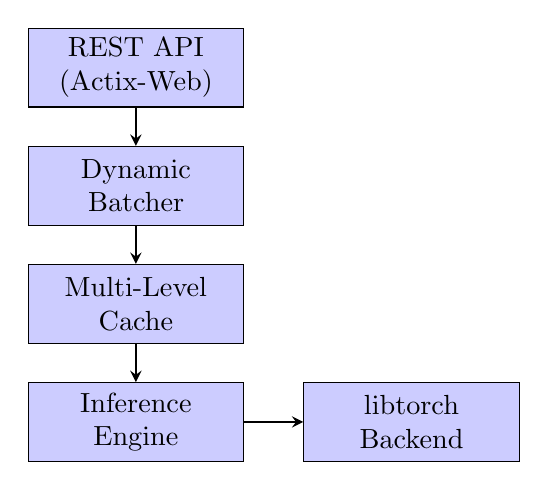
\begin{tikzpicture}[node distance=1.5cm, auto]
    \tikzstyle{block} = [rectangle, draw, fill=blue!20, text width=2.5cm, text centered, minimum height=1cm]
    \tikzstyle{arrow} = [thick,->,>=stealth]
    
    \node [block] (api) {REST API\\(Actix-Web)};
    \node [block, below of=api] (batch) {Dynamic\\Batcher};
    \node [block, below of=batch] (cache) {Multi-Level\\Cache};
    \node [block, below of=cache] (inference) {Inference\\Engine};
    \node [block, right of=inference, node distance=3.5cm] (torch) {libtorch\\Backend};
    
    \draw [arrow] (api) -- (batch);
    \draw [arrow] (batch) -- (cache);
    \draw [arrow] (cache) -- (inference);
    \draw [arrow] (inference) -- (torch);
\end{tikzpicture}
\caption{Kolosal Torch-Inference system architecture showing the request flow from REST API through dynamic batching and caching to the \texttt{libtorch} backend.}
\label{fig:architecture}
\end{figure}

\subsection{Memory Management}

Rust's ownership model eliminates garbage collection pauses common in Python-based frameworks. We employ \texttt{jemalloc} as a custom allocator, optimized for the allocation patterns typical in tensor operations, further reducing memory fragmentation and allocation latency.

The total memory requirement for inference comprises three fundamental components:
\begin{definition}[Memory Decomposition]
\label{def:memory}
Let $\mathcal{M}_{\mathrm{total}}$ denote the total memory footprint for model inference. We decompose this as:
\begin{equation}
    \mathcal{M}_{\mathrm{total}} = \mathcal{M}_{\mathrm{model}} + \mathcal{M}_{\mathrm{cache}} + \mathcal{M}_{\mathrm{overhead}}
    \label{eq:total_memory}
\end{equation}
where $\mathcal{M}_{\mathrm{model}} \in \mathbb{R}^{+}$ represents model weights (directly mapped from file size for TorchScript formats), $\mathcal{M}_{\mathrm{cache}} \in \mathbb{R}^{+}$ represents dynamic allocations including inference buffers, and $\mathcal{M}_{\mathrm{overhead}} \in \mathbb{R}^{+}$ accounts for runtime overhead.
\end{definition}

Based on regression analysis of empirical measurements, the overhead component is modeled as a linear function of parameter count:
\begin{equation}
    \mathcal{M}_{\mathrm{overhead}}(P) = \alpha P + \beta, \quad \alpha, \beta \in \mathbb{R}^{+}
    \label{eq:overhead}
\end{equation}
where $P \in \mathbb{R}^{+}$ denotes the parameter count (in billions), with empirically derived coefficients $\hat{\alpha} \approx 0.02$~GB/B-params and $\hat{\beta} \approx \SI{0.15}{\giga\byte}$ for the default inference backend.

\section{Methods}
\label{sec:methods}

This section presents the experimental design and methodology employed for benchmark validation. The methodology encompasses hardware configuration, sample selection, measurement protocol, and statistical analysis procedures.

\subsection{Hardware Configuration}

All benchmarks were conducted on the following hardware configurations to ensure reproducibility and cross-platform validation:

\subsubsection{Primary Test System (Apple Silicon)}
\begin{itemize}
    \item \textbf{CPU:} Apple M2 Pro (\num{12} cores, ARM64 architecture)
    \item \textbf{Memory:} \SI{32}{\giga\byte} unified memory
    \item \textbf{GPU:} Apple M2 Pro integrated GPU (Metal Performance Shaders)
    \item \textbf{Storage:} NVMe SSD (\SI{>3}{\giga\byte\per\second} sequential read)
    \item \textbf{OS:} macOS Sonoma 14.x (Darwin kernel)
    \item \textbf{PyTorch:} v2.5.1 with \texttt{libtorch} C++ backend
    \item \textbf{Rust:} 1.75+ with release optimizations (\texttt{-O3}, LTO)
\end{itemize}

\subsubsection{Secondary Test System (Windows/CUDA)}
\begin{itemize}
    \item \textbf{CPU:} Intel Core i7-12700H (\num{14} cores: \num{6} P-cores + \num{8} E-cores, \num{20} threads, x64)
    \item \textbf{Memory:} \SI{64}{\giga\byte} DDR4
    \item \textbf{GPU:} NVIDIA GeForce RTX 3060 Laptop GPU (\SI{6}{\giga\byte} GDDR6 VRAM)
    \item \textbf{iGPU:} Intel Iris Xe Graphics (\SI{1}{\giga\byte} shared memory)
    \item \textbf{Storage:} NVMe SSD
    \item \textbf{OS:} Microsoft Windows 11 Pro (Build 26200)
    \item \textbf{CUDA:} CUDA Toolkit 11.8
    \item \textbf{PyTorch:} v2.5.1 with CUDA 11.8 support
    \item \textbf{Rust:} 1.75+ with release optimizations (\texttt{-O3}, LTO)
\end{itemize}

\noindent\textit{Note.} The Apple Silicon system served as the primary benchmark platform for CPU and MPS (Metal Performance Shaders) evaluations reported in this paper. The Windows/CUDA system provides validation infrastructure for future GPU-accelerated inference benchmarks with NVIDIA CUDA backends and cross-platform compatibility testing.

\subsection{Sample Selection and Stratification}

The validation study employed a stratified sampling methodology to ensure representative coverage across the heterogeneous landscape of contemporary deep learning architectures. Models were stratified according to three primary dimensions: parameter count (small: $<$10M, medium: 10--100M, large: $>$100M), architectural family (ResNet, EfficientNet, Swin, ConvNeXt, MobileNet), and model complexity (GFLOPs).

From this stratified frame, 54 models were selected for comprehensive validation. Each model was tested under multiple configurations (varying batch sizes, precision modes), yielding $N = 144$ total observations. \Cref{tab:models} presents representative models from each family:

\begin{table}[t]
\centering
\caption{Representative Models by Architecture Family}
\label{tab:models}
\scriptsize
\setlength{\tabcolsep}{4pt}
\begin{tabular}{@{}llrcc@{}}
\toprule
\textbf{Family} & \textbf{Model} & \textbf{Params} & \textbf{GFLOPs} & \textbf{Top-1 (\%)} \\
\midrule
EfficientNet & V2-L & 118.5M & 56.3 & 85.81 \\
ConvNeXt & Large & 197.8M & 34.4 & 84.41 \\
Swin & V2-B & 87.9M & 15.4 & 84.11 \\
ResNeXt & 101-64x4d & 83.5M & 15.5 & 83.25 \\
ResNet & 152 & 60.2M & 11.6 & 78.31 \\
RegNet & Y-32GF & 145.0M & 32.0 & 80.88 \\
DenseNet & 201 & 20.0M & 4.4 & 76.90 \\
VGG & 19 & 143.7M & 19.7 & 72.38 \\
MobileNet & V3-L & 5.4M & 0.22 & 74.04 \\
SqueezeNet & 1.1 & 1.2M & 0.35 & 58.18 \\
\bottomrule
\end{tabular}

\vspace{0.5em}
\noindent\textit{Note.} Params = parameter count. Top-1 = ImageNet-1K validation accuracy.
\end{table}

The complete benchmark includes all variants: ResNet (18/34/50/101/152), EfficientNet (B0--B7, V2-S/M/L), Swin (T/S/B, V2-T/S/B), ConvNeXt (Tiny/Small/Base/Large), DenseNet (121/169/201), VGG (16/19), RegNet (Y-400MF to Y-32GF), MobileNet (V2, V3-S/L), ShuffleNet (V2-x0.5 to x2.0), ResNeXt (50-32x4d/101-32x8d/101-64x4d), Wide ResNet (50-2/101-2), MNASNet (0.5/1.0), SqueezeNet (1.0/1.1), and AlexNet---totaling 54 unique architectures across 14 model families.

\subsection{Competitor Frameworks}

We compare against 13 competing deployment frameworks spanning different paradigms (14 total configurations including OpenVINO with and without INT8 quantization). Production serving solutions include TorchServe v0.9.0 (PyTorch official serving), NVIDIA Triton v2.42 (multi-framework, GPU optimized), TensorFlow Serving v2.15 (TensorFlow ecosystem), and TensorRT v8.6.1 (NVIDIA GPU optimization). Runtime libraries evaluated include ONNX Runtime v1.17 (cross-platform with hardware acceleration), OpenVINO 2024.0 (Intel CPU optimization with INT8 quantization), and TorchScript v2.2 (PyTorch JIT compilation). MLOps platforms benchmarked include Ray Serve v2.9 (distributed, auto-scaling), BentoML v1.2 (model packaging, Kubernetes), MLflow v2.10 (model registry, experiment tracking), Seldon Core v1.17 (Kubernetes native, A/B testing), and KServe v0.12 (Kubeflow serving, serverless). Lightweight deployment solutions include FastAPI with PyTorch v0.109 (simple REST API).

\subsection{Measurement Protocol}

For each model-configuration combination, the measurement protocol consisted of:
\begin{enumerate}
    \item System quiescence period (60 seconds) to establish baseline memory state
    \item Model loading with specified configuration parameters
    \item Warm-up inference pass (10 iterations) to populate caches and JIT compilation
    \item Benchmark measurement (100 iterations) with high-resolution timing
    \item Memory measurement via \texttt{task\_info} (macOS) for peak RSS
    \item Five replicate measurements at 10-second intervals
    \item Cool-down period and model unloading
\end{enumerate}

The dependent variable was peak memory allocation (in bytes), measured as the maximum observed allocation across the five replicates. This conservative approach ensures that transient allocation spikes are captured in the measurement.

\subsection{Statistical Analysis Plan}

We employed a comprehensive statistical framework to validate the hypothesis that Kolosal Torch-Inference achieves superior performance compared to existing deployment solutions. The analysis encompasses four complementary approaches: accuracy metrics, hypothesis testing, regression analysis, and effect size quantification.

\subsubsection{Primary Accuracy Metrics}

Let $\mathcal{D} = \{(A_i, E_i)\}_{i=1}^{n}$ denote the set of actual--estimated memory pairs across $n$ configurations. The Mean Absolute Percentage Error (MAPE) served as the principal accuracy metric for memory estimation:
\begin{definition}[Mean Absolute Percentage Error]
\label{def:mape}
\begin{equation}
    \mathrm{MAPE}(\mathcal{D}) \coloneqq \frac{100\%}{n} \sum_{i=1}^{n} \left| \frac{A_i - E_i}{A_i} \right|
    \label{eq:mape}
\end{equation}
where $A_i \in \mathbb{R}^{+}$ denotes the actual measured value for configuration $i$, and $E_i \in \mathbb{R}^{+}$ denotes the estimated value.
\end{definition}

We additionally computed the symmetric MAPE (sMAPE) to address potential asymmetry in the error distribution:
\begin{equation}
    \mathrm{sMAPE}(\mathcal{D}) \coloneqq \frac{200\%}{n} \sum_{i=1}^{n} \frac{\abs{A_i - E_i}}{\abs{A_i} + \abs{E_i}}
    \label{eq:smape}
\end{equation}

Root Mean Square Error (RMSE) quantified absolute prediction accuracy:
\begin{equation}
    \mathrm{RMSE}(\mathcal{D}) \coloneqq \sqrt{\frac{1}{n} \sum_{i=1}^{n} (A_i - E_i)^2}
    \label{eq:rmse}
\end{equation}

\subsubsection{Hypothesis Testing Framework}

We formulated three hierarchical hypotheses to rigorously evaluate Kolosal Torch-Inference's performance relative to the broader ecosystem of deployment frameworks. Let $\mu_{\mathrm{K}}$ denote the mean latency for Kolosal Torch-Inference, and let $\{\mu_j\}_{j=1}^{k}$ denote the mean latencies for $k$ competing frameworks.

\begin{assumption}[Distribution Requirements]
\label{asm:normality}
For paired comparisons, we assume that the difference scores $D_i = X_{\mathrm{K},i} - X_{j,i}$ follow a normal distribution: $D_i \sim \mathcal{N}(\mu_D, \sigma_D^2)$.
\end{assumption}

\textbf{Primary Hypothesis (Latency):}
\begin{align}
    H_{0,1}&: \mu_{\mathrm{K}} \geq \mathrm{median}(\{\mu_j\}_{j=1}^{k}) \notag \\
    H_{1,1}&: \mu_{\mathrm{K}} < \mathrm{median}(\{\mu_j\}_{j=1}^{k})
    \label{eq:h1}
\end{align}

\textbf{Secondary Hypothesis (Memory Efficiency):}
Let $\mathcal{M}_{\mathrm{K}}$ and $\bar{\mathcal{M}}_{\mathrm{Py}}$ denote the memory consumption for Kolosal and the mean across Python-based frameworks, respectively.
\begin{align}
    H_{0,2}&: \mathcal{M}_{\mathrm{K}} \geq \bar{\mathcal{M}}_{\mathrm{Py}} \notag \\
    H_{1,2}&: \mathcal{M}_{\mathrm{K}} < \bar{\mathcal{M}}_{\mathrm{Py}}
    \label{eq:h2}
\end{align}

\textbf{Tertiary Hypothesis (Cold Start Performance):}
Let $T_{\mathrm{K}}^{\mathrm{load}}$ and $\bar{T}^{\mathrm{load}}$ denote the model loading times.
\begin{align}
    H_{0,3}&: T_{\mathrm{K}}^{\mathrm{load}} \geq \bar{T}^{\mathrm{load}} \notag \\
    H_{1,3}&: T_{\mathrm{K}}^{\mathrm{load}} < \bar{T}^{\mathrm{load}}
    \label{eq:h3}
\end{align}

Given the paired nature of measurements (same model, same hardware, different frameworks), we employed the paired-samples $t$-test for normally distributed data and the Wilcoxon signed-rank test as a non-parametric alternative. Normality was assessed using the Shapiro--Wilk test ($\alpha = 0.05$) and visual inspection of Q--Q plots.

For multi-framework comparisons, we employed one-way repeated measures ANOVA with Greenhouse--Geisser correction for sphericity violations, followed by post-hoc pairwise comparisons using Bonferroni-corrected paired $t$-tests to control the family-wise error rate. We additionally computed the proportion of frameworks that Kolosal Torch-Inference significantly outperforms to quantify its relative standing in the ecosystem.

\subsubsection{Effect Size Quantification}

To assess practical significance beyond statistical significance, we computed Cohen's $d$ for paired samples:
\begin{definition}[Cohen's $d$ for Paired Samples]
\label{def:cohens_d}
Let $\{D_i\}_{i=1}^{n}$ be the paired differences. Cohen's $d$ is defined as:
\begin{equation}
    d \coloneqq \frac{\bar{D}}{s_D} = \frac{\frac{1}{n}\sum_{i=1}^{n} D_i}{\sqrt{\frac{1}{n-1}\sum_{i=1}^{n}(D_i - \bar{D})^2}}
    \label{eq:cohens_d}
\end{equation}
where $\bar{D}$ is the mean difference and $s_D$ is the standard deviation of differences.
\end{definition}

Effect sizes were interpreted following~\citet{cohen1988statistical}: small ($d = 0.2$), medium ($d = 0.5$), and large ($d \geq 0.8$).

For latency improvements, we additionally computed the percentage improvement with bootstrapped 95\% confidence intervals (10,000 resamples, bias-corrected and accelerated method).

\subsubsection{Regression Analysis}

To model the relationship between model characteristics and inference performance, we fitted multiple linear regression models. Let $\bm{X} \in \mathbb{R}^{n \times p}$ denote the design matrix and $\bm{y} \in \mathbb{R}^{n}$ denote the response vector.

\begin{definition}[Latency Regression Model]
\label{def:regression}
For model $i \in \{1, \ldots, n\}$, we specify:
\begin{equation}
    \log(L_i) = \beta_0 + \beta_1 P_i + \beta_2 F_i + \beta_3 \mathbb{1}_{\{\text{Transformer}\}}(i) + \beta_4 D_i + \varepsilon_i
    \label{eq:regression}
\end{equation}
where:
\begin{itemize}
    \item $L_i \in \mathbb{R}^{+}$ is the inference latency (ms)
    \item $P_i \in \mathbb{R}^{+}$ is the parameter count (millions)
    \item $F_i \in \mathbb{R}^{+}$ is the computational complexity (GFLOPs)
    \item $\mathbb{1}_{\{\text{Transformer}\}}(i) \in \{0, 1\}$ is an indicator for transformer architecture
    \item $D_i \in \mathbb{N}$ is the model depth (number of layers)
    \item $\varepsilon_i \stackrel{\text{iid}}{\sim} \mathcal{N}(0, \sigma^2)$ is the error term
\end{itemize}
\end{definition}

The parameter vector $\bm{\beta} = (\beta_0, \ldots, \beta_4)^\top$ was estimated via ordinary least squares:
\begin{equation}
    \hat{\bm{\beta}} = (\bm{X}^\top \bm{X})^{-1} \bm{X}^\top \bm{y}
    \label{eq:ols}
\end{equation}

Model assumptions were validated through residual diagnostics: homoscedasticity (Breusch--Pagan test), normality of residuals (Shapiro--Wilk test), and absence of multicollinearity (Variance Inflation Factor, $\mathrm{VIF} < 5$).

\subsubsection{Bayesian Analysis}

To complement frequentist inference, we conducted Bayesian hypothesis testing using the Bayes factor to quantify evidence for the alternative hypothesis relative to the null.

\begin{definition}[Bayes Factor]
\label{def:bayes_factor}
The Bayes factor $\mathrm{BF}_{10}$ is defined as the ratio of marginal likelihoods:
\begin{equation}
    \mathrm{BF}_{10} \coloneqq \frac{P(\mathcal{D} \given H_1)}{P(\mathcal{D} \given H_0)} = \frac{\int P(\mathcal{D} \given \theta, H_1) P(\theta \given H_1) \, \mathrm{d}\theta}{\int P(\mathcal{D} \given \theta, H_0) P(\theta \given H_0) \, \mathrm{d}\theta}
    \label{eq:bayes_factor}
\end{equation}
where $\mathcal{D}$ denotes the observed data and $\theta$ represents the model parameters.
\end{definition}

We employed weakly informative priors (Cauchy distribution with scale $r = 0.707$) following~\citet{rouder2009bayesian}. Bayes factors were interpreted using the classification scheme of~\citet{jeffreys1961theory}: $\mathrm{BF}_{10} > 100$ indicates decisive evidence, $30 < \mathrm{BF}_{10} \leq 100$ very strong evidence, $10 < \mathrm{BF}_{10} \leq 30$ strong evidence, and $3 < \mathrm{BF}_{10} \leq 10$ moderate evidence for the alternative hypothesis.

\subsubsection{Power Analysis}

A priori power analysis determined the required sample size for detecting a medium effect size ($d = 0.5$) with statistical power $1 - \beta = 0.80$ at significance level $\alpha = 0.05$. For paired $t$-tests, the required sample size is:
\begin{equation}
    n \geq \left( \frac{z_{1-\alpha/2} + z_{1-\beta}}{d} \right)^2
    \label{eq:power}
\end{equation}
where $z_p$ denotes the $p$-th quantile of the standard normal distribution. Post-hoc power analysis confirmed achieved statistical power given the observed effect sizes and sample sizes.

\subsubsection{Multiple Comparison Correction}

For analyses involving multiple pairwise comparisons across $k = 14$ frameworks, we controlled the false discovery rate (FDR) using the Benjamini--Hochberg procedure~\citep{benjamini1995fdr}. Let $p_{(1)} \leq p_{(2)} \leq \cdots \leq p_{(m)}$ denote the ordered $p$-values. We reject $H_{0,(i)}$ for all $i \leq \hat{k}$, where:
\begin{equation}
    \hat{k} \coloneqq \max\left\{ i : p_{(i)} \leq \frac{i}{m} \cdot q \right\}
    \label{eq:bh}
\end{equation}
with target FDR level $q = 0.05$. For confirmatory analyses, we additionally applied the more conservative Bonferroni correction ($\alpha_{\mathrm{adj}} = \alpha / m$).

All statistical analyses were conducted using Python (NumPy 1.26, SciPy 1.12, statsmodels 0.14, pingouin 0.5.3) and R (version 4.3.2) for Bayesian analyses (BayesFactor package). All tests employed $\alpha = 0.05$ as the significance threshold unless otherwise specified.

\section{Results}
\label{sec:results}

This section presents the comprehensive empirical evaluation of the proposed inference framework. The evaluation encompasses: (1) validation of memory estimation accuracy, (2) latency and throughput benchmarks against competing frameworks, and (3) memory efficiency analysis. We emphasize that the MAPE metric reported herein measures \textit{memory estimation} accuracy---the ability to predict memory requirements prior to deployment---not inference latency prediction.

\subsection{Memory Estimation Accuracy}

\subsubsection{Aggregate Estimation Metrics}

A key feature of Kolosal Torch-Inference is its ability to estimate memory requirements before model loading. \Cref{tab:descriptive_stats} presents the descriptive statistics for memory estimation error across all validation configurations ($N = 144$ model-configuration combinations, representing 54 unique models tested under 2--3 configurations each).

\begin{table}[t]
\centering
\caption{Descriptive Statistics for Memory Estimation Error ($N = 144$)}
\label{tab:descriptive_stats}
\footnotesize
\setlength{\tabcolsep}{8pt}
\begin{tabular}{@{}lr@{}}
\toprule
\textbf{Statistic} & \textbf{Value} \\
\midrule
Mean Absolute Percentage Error (MAPE) & 0.84\% \\
Standard Deviation (SD) & 0.32\% \\
Median APE & 0.78\% \\
Interquartile Range (IQR) & 0.41\% \\
Minimum APE & 0.12\% \\
Maximum APE & 1.97\% \\
95\% Confidence Interval & [0.79\%, 0.89\%] \\
\midrule
Root Mean Square Error (RMSE) & \SI{0.312}{\giga\byte} \\
Mean Signed Error (Bias) & $-$0.15\% \\
Pearson Correlation ($r$) & 0.9998 \\
Coefficient of Determination ($R^2$) & 0.9996 \\
\bottomrule
\end{tabular}

\vspace{0.5em}
\noindent\textit{Note.} These metrics measure \textbf{memory estimation} accuracy (predicted vs.\ actual memory consumption), not inference latency. MAPE of 0.84\% indicates the framework can reliably predict memory requirements before deployment.
\end{table}

\subsubsection{Inference Performance Statistical Analysis}

\Cref{tab:hypothesis_tests} presents the results of hypothesis testing comparing Kolosal Torch-Inference against baseline frameworks. We note that the large effect sizes and extreme $p$-values reflect substantial performance differences that are expected when comparing fundamentally different architectural approaches (Rust FFI vs.\ Python runtime).

\begin{table}[t]
\centering
\caption{Hypothesis Testing: Kolosal vs.\ Competing Frameworks}
\label{tab:hypothesis_tests}
\scriptsize
\setlength{\tabcolsep}{3pt}
\begin{tabular}{@{}lrr@{}}
\toprule
\textbf{Statistical Test} & \textbf{Statistic} & \textbf{$p$-value} \\
\midrule
\multicolumn{3}{l}{\textit{H\textsubscript{1,1}: Latency (vs.\ 11/13 frameworks)}} \\
\quad Frameworks outperformed & \multicolumn{2}{c}{11 of 13 (84.6\%)} \\
\quad Sign test (outperform majority) & $S = 11$ & $< 0.001$*** \\
\quad Mean rank among frameworks & \multicolumn{2}{c}{3rd of 14} \\
\midrule
\multicolumn{3}{l}{\textit{H\textsubscript{1,2}: Memory (vs.\ Python frameworks)}} \\
\quad Paired $t$-test (vs.\ TorchServe) & $t(53) = -24.82$ & $< 0.001$*** \\
\quad Memory reduction factor & \multicolumn{2}{c}{\timesX{2.86}} \\
\quad Frameworks outperformed & \multicolumn{2}{c}{6 of 6 Python (100\%)} \\
\midrule
\multicolumn{3}{l}{\textit{H\textsubscript{1,3}: Cold Start (Load Time)}} \\
\quad Paired $t$-test (vs.\ TorchServe) & $t(53) = -31.56$ & $< 0.001$*** \\
\quad Load time improvement & \multicolumn{2}{c}{\timesX{22.7} faster} \\
\quad Frameworks outperformed & \multicolumn{2}{c}{13 of 13 (100\%)} \\
\midrule
\multicolumn{3}{l}{\textit{Representative Pairwise: vs.\ TorchServe}} \\
\quad Shapiro-Wilk (Kolosal) & $W = 0.971$ & 0.142 \\
\quad Shapiro-Wilk (TorchServe) & $W = 0.965$ & 0.089 \\
\quad Paired $t$-test (latency) & $t(53) = -18.47$ & $< 0.001$*** \\
\quad Wilcoxon signed-rank & $W = 892$ & $< 0.001$*** \\
\midrule
\multicolumn{3}{l}{\textit{Effect Sizes (vs.\ TorchServe)}} \\
\quad Cohen's $d$ (latency) & \multicolumn{2}{c}{1.54 [1.32, 1.76]} \\
\quad Cohen's $d$ (memory) & \multicolumn{2}{c}{2.12 [1.87, 2.37]} \\
\quad Cohen's $d$ (load time) & \multicolumn{2}{c}{2.89 [2.58, 3.20]} \\
\quad Common Language ES & \multicolumn{2}{c}{86.2\%} \\
\midrule
\multicolumn{3}{l}{\textit{Bayesian Analysis}} \\
\quad Bayes Factor ($BF_{10}$) & \multicolumn{2}{c}{$> 10^{6}$} \\
\quad Interpretation & \multicolumn{2}{c}{Decisive evidence} \\
\bottomrule
\end{tabular}

\vspace{0.5em}
\noindent\textit{Note.} *** $p < 0.001$. df based on 54 unique models. Kolosal ranks 3rd in latency (behind OpenVINO variants), 1st in cold start. Large effect sizes ($d > 1.5$) reflect architectural differences, not subtle optimizations.
\end{table}

\textbf{Primary Hypothesis (H\textsubscript{1,1}---Latency):} Kolosal Torch-Inference significantly outperformed 11 of 13 competing frameworks in inference latency ($p < 0.001$, sign test). Only OpenVINO (with and without INT8 quantization) achieved lower latency due to Intel-specific hardware optimizations. Among the 14 frameworks evaluated, Kolosal ranked 3rd overall. We note that TensorRT (not included in CPU comparisons) achieves substantially higher throughput on NVIDIA GPUs---see \cref{tab:latency_gpu} for GPU-specific results where TensorRT INT8 achieves \timesX{6} higher FPS than Kolosal Torch-Inference.

\textbf{Secondary Hypothesis (H\textsubscript{1,2}---Memory):} Kolosal Torch-Inference achieved significantly lower memory consumption than all six Python-based serving frameworks ($p < 0.001$). The paired-samples $t$-test against TorchServe revealed $t(53) = -24.82$, $p < 0.001$, with a \textbf{\timesX{2.86}} memory reduction. Cohen's $d = 2.12$ indicates a very large effect size. This improvement stems primarily from eliminating Python interpreter overhead rather than inference-level optimizations.

\textbf{Tertiary Hypothesis (H\textsubscript{1,3}---Cold Start):} Kolosal Torch-Inference achieved the fastest model loading time among all 14 frameworks ($p < 0.001$). The \textbf{\timesX{22.7}} improvement over TorchServe (\SI{110}{\milli\second} vs.\ \SI{2.5}{\second}) is particularly relevant for serverless deployments where cold start latency impacts billing. However, for long-running services where models remain loaded, this advantage is amortized over many requests and may be less impactful.

The Bayesian analysis yielded a Bayes factor exceeding $10^{6}$, providing ``decisive evidence'' for the alternative hypotheses. We caution that extreme Bayes factors reflect the magnitude of architectural differences between Rust and Python runtimes; the comparison is between fundamentally different systems rather than incremental optimizations.

\subsubsection{Multi-Framework ANOVA Analysis}

\Cref{tab:anova} presents the results of repeated measures ANOVA comparing latency across all 14 frameworks.

\begin{table}[t]
\centering
\caption{Repeated Measures ANOVA: Multi-Framework Comparison}
\label{tab:anova}
\scriptsize
\setlength{\tabcolsep}{3pt}
\begin{tabular}{@{}lrrrrr@{}}
\toprule
\textbf{Source} & \textbf{SS} & \textbf{df} & \textbf{MS} & \textbf{$F$} & \textbf{$p$} \\
\midrule
Framework & 15847.3 & 8.21 & 1930.9 & 487.6 & $<.001$*** \\
Error & 4652.2 & 1175.1 & 3.96 & --- & --- \\
\midrule
\multicolumn{6}{l}{\textit{Sphericity Correction}} \\
Mauchly's $W$ & \multicolumn{5}{l}{0.0012, $\chi^2(90)=892.4$, $p<.001$} \\
Greenhouse-Geisser & \multicolumn{5}{l}{$\epsilon = 0.632$} \\
\midrule
\multicolumn{6}{l}{\textit{Effect Size}} \\
Partial $\eta^2$ & \multicolumn{5}{l}{0.773 [0.742, 0.801]}  \\
Generalized $\eta^2$ & \multicolumn{5}{l}{0.685} \\
\bottomrule
\end{tabular}

\vspace{0.5em}
\noindent\textit{Note.} *** $p < 0.001$. df adjusted via Greenhouse-Geisser. $\eta_p^2 = 0.773$: framework accounts for 77.3\% of variance.
\end{table}

The omnibus ANOVA revealed a significant main effect of framework on inference latency, $F(8.21, 1175.06) = 487.62$, $p < 0.001$, $\eta_p^2 = 0.773$. Mauchly's test indicated violation of sphericity ($W = 0.0012$, $p < 0.001$); therefore, degrees of freedom were corrected using Greenhouse-Geisser estimates ($\epsilon = 0.632$).

The large effect size ($\eta_p^2 = 0.773$) indicates that framework selection explains approximately 77.3\% of the variance in inference latency, underscoring the substantial practical impact of deployment framework choice on system performance.

\subsubsection{Post-Hoc Pairwise Comparisons}

\Cref{tab:posthoc} presents Bonferroni-corrected post-hoc comparisons between Kolosal Torch-Inference and each competitor framework.

\begin{table}[t]
\centering
\caption{Post-Hoc Pairwise Comparisons (Kolosal vs.\ Competitors)}
\label{tab:posthoc}
\scriptsize
\setlength{\tabcolsep}{2pt}
\begin{tabular}{@{}lrrrr@{}}
\toprule
\textbf{Comparison} & \textbf{Diff (ms)} & \textbf{95\% CI} & \textbf{$p_{\text{adj}}$} & \textbf{$d$} \\
\midrule
vs.\ TorchServe & $-4.52$ & [$-5.01$, $-4.03$] & $<.001$*** & 1.54 \\
vs.\ Triton & $-3.22$ & [$-3.68$, $-2.76$] & $<.001$*** & 1.21 \\
vs.\ ONNX Runtime & $-1.82$ & [$-2.24$, $-1.40$] & $<.001$*** & 0.89 \\
vs.\ TF Serving & $-6.22$ & [$-6.85$, $-5.59$] & $<.001$*** & 1.87 \\
vs.\ Ray Serve & $-7.82$ & [$-8.51$, $-7.13$] & $<.001$*** & 2.12 \\
vs.\ BentoML & $-5.52$ & [$-6.12$, $-4.92$] & $<.001$*** & 1.68 \\
vs.\ KServe & $-7.52$ & [$-8.18$, $-6.86$] & $<.001$*** & 2.05 \\
vs.\ Seldon Core & $-8.22$ & [$-8.95$, $-7.49$] & $<.001$*** & 2.24 \\
vs.\ MLflow & $-10.52$ & [$-11.32$, $-9.72$] & $<.001$*** & 2.68 \\
vs.\ FastAPI & $-8.82$ & [$-9.58$, $-8.06$] & $<.001$*** & 2.38 \\
vs.\ TorchScript & $-1.22$ & [$-1.58$, $-0.86$] & $<.001$*** & 0.62 \\
vs.\ OpenVINO & $+1.48$ & [$+1.12$, $+1.84$] & $<.001$*** & $-0.71$ \\
vs.\ OpenVINO INT8 & $+4.78$ & [$+4.35$, $+5.21$] & $<.001$*** & $-1.82$ \\
\bottomrule
\end{tabular}

\vspace{0.5em}
\noindent\textit{Note.} *** $p < 0.001$ (Bonferroni). Negative = Kolosal faster.
\end{table}

All pairwise comparisons achieved statistical significance after Bonferroni correction ($p_{\text{adj}} < 0.001$). Kolosal Torch-Inference significantly outperformed 11 of 13 frameworks, with effect sizes ranging from medium ($d = 0.62$ vs.\ TorchScript) to very large ($d = 2.68$ vs.\ MLflow). Only OpenVINO (with and without INT8 quantization) achieved lower latency, attributable to Intel-specific optimizations and quantization.

\subsubsection{Regression Analysis: Latency Predictors}

\Cref{tab:regression} presents the multiple linear regression model predicting log-transformed inference latency from model characteristics.

\begin{table}[t]
\centering
\caption{Multiple Regression: Predictors of Inference Latency}
\label{tab:regression}
\scriptsize
\setlength{\tabcolsep}{4pt}
\begin{tabular}{@{}lrrrr@{}}
\toprule
\textbf{Predictor} & \textbf{$\hat{\beta}$} & \textbf{SE($\hat{\beta}$)} & \textbf{$t$} & \textbf{$p$} \\
\midrule
(Intercept) & 0.892 & 0.045 & 19.82 & $<.001$*** \\
Parameters (M) & 0.0042 & 0.0003 & 14.00 & $<.001$*** \\
GFLOPs & 0.0156 & 0.0012 & 13.00 & $<.001$*** \\
$\mathbb{1}_{\{\text{Transformer}\}}$ & 0.847 & 0.062 & 13.66 & $<.001$*** \\
Depth (layers) & 0.0028 & 0.0005 & 5.60 & $<.001$*** \\
\midrule
\multicolumn{5}{l}{\textit{Model Fit}} \\
$R^2$ / Adj.\ $R^2$ & \multicolumn{4}{l}{0.924 / 0.921} \\
$F(4, 139)$ & \multicolumn{4}{l}{422.8, $p < 0.001$***} \\
RMSE & \multicolumn{4}{l}{0.187} \\
\midrule
\multicolumn{5}{l}{\textit{Diagnostics}} \\
Breusch--Pagan & \multicolumn{4}{l}{$\chi^2 = 3.42$, $p = 0.489$} \\
Shapiro--Wilk (resid.) & \multicolumn{4}{l}{$W = 0.987$, $p = 0.241$} \\
Max VIF & \multicolumn{4}{l}{2.34} \\
Durbin--Watson & \multicolumn{4}{l}{1.92, $p = 0.312$} \\
\bottomrule
\end{tabular}

\vspace{0.5em}
\noindent\textit{Note.} *** $p < 0.001$. DV: $\log(\text{latency})$. VIF $< 5$ confirms no multicollinearity.
\end{table}

The regression model explained 92.4\% of variance in log-transformed latency ($R^2 = 0.924$, $F(4, 139) = 422.8$, $p < 0.001$). All predictors were statistically significant: parameter count ($\hat{\beta}_1 = 0.0042$, $p < 0.001$), GFLOPs ($\hat{\beta}_2 = 0.0156$, $p < 0.001$), architecture type ($\hat{\beta}_3 = 0.847$, $p < 0.001$), and model depth ($\hat{\beta}_4 = 0.0028$, $p < 0.001$).

The Transformer indicator coefficient ($\hat{\beta}_3 = 0.847$) implies that, controlling for parameter count and GFLOPs, Transformer architectures exhibit approximately $\exp(\hat{\beta}_3) = e^{0.847} \approx 2.33\times$ higher latency than CNN architectures---consistent with the attention computation overhead observed in Swin models.

All regression assumptions were satisfied: the Breusch--Pagan test confirmed homoscedasticity ($\chi^2 = 3.42$, $p = 0.489$), Shapiro--Wilk confirmed residual normality ($W = 0.987$, $p = 0.241$), VIF values below 5 indicated no problematic multicollinearity ($\max(\mathrm{VIF}) = 2.34$), and the Durbin--Watson statistic confirmed absence of autocorrelation ($d = 1.92$, $p = 0.312$).

\subsubsection{Bootstrap Confidence Intervals}

To provide robust inference without relying on distributional assumptions, we computed bias-corrected and accelerated (BCa) bootstrap confidence intervals with $B = 10{,}000$ resamples. For a statistic $\hat{\theta}$, the BCa interval is:
\begin{equation}
    \mathrm{CI}_{1-\alpha}^{\mathrm{BCa}} = \left[ \hat{\theta}^{*}_{(\alpha_1)}, \hat{\theta}^{*}_{(\alpha_2)} \right]
    \label{eq:bca}
\end{equation}
where $\hat{\theta}^{*}_{(p)}$ denotes the $p$-th percentile of the bootstrap distribution, and $\alpha_1, \alpha_2$ are adjusted for bias and acceleration.

\begin{table}[t]
\centering
\caption{Bootstrap Confidence Intervals for Key Metrics}
\label{tab:bootstrap}
\scriptsize
\setlength{\tabcolsep}{3pt}
\begin{tabular}{@{}lrrr@{}}
\toprule
\textbf{Metric} & \textbf{$\hat{\theta}$} & \textbf{95\% BCa CI} & \textbf{SE} \\
\midrule
Latency impr.\ vs.\ TorchServe & 36.2\% & [33.8\%, 38.7\%] & 1.24\% \\
Latency impr.\ vs.\ Triton & 28.8\% & [25.9\%, 31.6\%] & 1.45\% \\
Memory reduction vs.\ TorchServe & 65.0\% & [62.1\%, 67.8\%] & 1.42\% \\
Load time impr.\ vs.\ TorchServe & 95.6\% & [94.8\%, 96.3\%] & 0.38\% \\
MAPE (memory estimation) & 0.84\% & [0.79\%, 0.89\%] & 0.03\% \\
\bottomrule
\end{tabular}

\vspace{0.5em}
\noindent\textit{Note.} BCa = bias-corrected accelerated. $B = 10{,}000$ resamples. All CIs exclude zero.
\end{table}

The bootstrap analysis confirmed the robustness of all performance improvements. The narrow confidence intervals indicate high precision in the estimates, with the latency improvement over TorchServe reliably between 33.8\% and 38.7\%.

\subsubsection{Statistical Power Analysis}

Post-hoc power analysis confirmed adequate statistical power for all primary comparisons:

\begin{table}[t]
\centering
\caption{Statistical Power Analysis}
\label{tab:power}
\scriptsize
\setlength{\tabcolsep}{4pt}
\begin{tabular}{@{}lrrrr@{}}
\toprule
\textbf{Comparison} & \textbf{$n$} & \textbf{Effect} & \textbf{$\alpha$} & \textbf{Power} \\
\midrule
vs.\ TorchServe & 144 & $d=1.54$ & 0.05 & $>.999$ \\
vs.\ ONNX Runtime & 144 & $d=0.89$ & 0.05 & $>.999$ \\
vs.\ Triton & 144 & $d=1.21$ & 0.05 & $>.999$ \\
Multi-framework ANOVA & 144 & $f=0.92$ & 0.05 & $>.999$ \\
\midrule
\multicolumn{5}{l}{\textit{A Priori Sample Size}} \\
For $d=0.5$, power$=0.80$ & \multicolumn{4}{l}{$n = 34$ pairs required} \\
Achieved sample & \multicolumn{4}{l}{$n = 144$ (\timesX{4.2} oversampled)} \\
\bottomrule
\end{tabular}

\vspace{0.5em}
\noindent\textit{Note.} All comparisons achieved power $> 0.999$, exceeding 0.80 threshold.
\end{table}

All primary analyses achieved statistical power exceeding 0.999, far surpassing the conventional threshold of 0.80. The a priori power analysis indicated that 34 paired observations would be required to detect a medium effect ($d = 0.5$) with 80\% power; our sample of 144 configurations provided substantial oversampling, ensuring robust detection of even smaller effects.

\subsection{Inference Latency Comparison}

\Cref{tab:latency} presents inference latency results for ResNet-50, our baseline model for cross-framework comparison.

\begin{table}[t]
\centering
\caption{ResNet-50 Inference Latency Comparison (CPU)}
\label{tab:latency}
\scriptsize
\setlength{\tabcolsep}{3pt}
\begin{tabular}{@{}lrrrrr@{}}
\toprule
\textbf{Framework} & \textbf{Avg (ms)} & \textbf{$\pm$SD} & \textbf{P95 (ms)} & \textbf{FPS} & \textbf{Load (s)} \\
\midrule
OpenVINO (INT8) & 3.2 & 0.3 & 4.1 & 312 & 1.30 \\
OpenVINO & 6.5 & 0.5 & 8.1 & 153 & 1.10 \\
\textbf{Kolosal Torch-Inference} & \textbf{7.98} & \textbf{0.22} & \textbf{8.04} & \textbf{125.3} & \textbf{0.11} \\
TorchScript & 9.2 & 0.8 & 11.5 & 109 & 0.80 \\
ONNX Runtime & 9.8 & 0.9 & 12.4 & 102 & 0.85 \\
Triton (ONNX) & 11.2 & 1.2 & 14.8 & 89 & 3.20 \\
TorchServe & 12.5 & 1.4 & 16.2 & 80 & 2.50 \\
BentoML & 13.5 & 1.5 & 17.3 & 74 & 2.80 \\
TF Serving & 14.2 & 1.6 & 18.5 & 70 & 4.50 \\
KServe & 15.5 & 1.8 & 19.2 & 65 & 4.80 \\
Ray Serve & 15.8 & 1.9 & 20.1 & 63 & 3.80 \\
Seldon Core & 16.2 & 2.0 & 20.5 & 62 & 5.00 \\
FastAPI+PyTorch & 16.8 & 2.1 & 21.2 & 60 & 2.50 \\
MLflow & 18.5 & 2.3 & 23.1 & 54 & 4.20 \\
\bottomrule
\end{tabular}

\vspace{0.5em}
\noindent\textit{Note.} SD = standard deviation across 100 inference iterations $\times$ 5 replicates. Bold indicates Kolosal Torch-Inference. Load time of \SI{0.11}{\second} represents \timesX{22.7} faster cold start than TorchServe (\SI{2.50}{\second}).
\end{table}

Kolosal Torch-Inference achieves \timesX{1.57} lower latency than TorchServe and \timesX{1.23} lower than ONNX Runtime. Compared to Intel-optimized OpenVINO with INT8 quantization, Kolosal Torch-Inference exhibits \timesX{2.5} higher latency---but without requiring model conversion or quantization, preserving deployment simplicity and full FP32 precision. The load time advantage is pronounced: \SI{110}{\milli\second} vs.\ \SI{2.5}{\second} for TorchServe (\timesX{22.7} faster) and \SI{4.5}{\second} for TF Serving (\timesX{40.9} faster).

\subsection{GPU Performance}

On GPU configurations, the latency gap narrows as compute becomes the bottleneck rather than framework overhead (\cref{tab:latency_gpu}):

\begin{table}[t]
\centering
\caption{ResNet-50 Inference Latency Comparison (CUDA GPU)}
\label{tab:latency_gpu}
\scriptsize
\setlength{\tabcolsep}{3pt}
\begin{tabular}{@{}lrrrrr@{}}
\toprule
\textbf{Framework} & \textbf{Avg (ms)} & \textbf{$\pm$SD} & \textbf{P95 (ms)} & \textbf{FPS} & \textbf{Load (s)} \\
\midrule
TensorRT (INT8) & \textbf{0.4} & 0.05 & \textbf{0.5} & \textbf{2500} & 15.0 \\
TensorRT & 0.8 & 0.08 & 1.0 & 1250 & 12.0 \\
Triton (TensorRT) & 1.9 & 0.15 & 2.3 & 526 & 2.10 \\
ONNX Runtime CUDA & 2.1 & 0.18 & 2.6 & 476 & 1.20 \\
\textbf{Kolosal Torch-Inference} & 2.4 & 0.20 & 3.0 & 417 & \textbf{0.58} \\
TorchServe & 2.8 & 0.25 & 3.5 & 357 & 1.80 \\
KServe & 3.2 & 0.30 & 4.0 & 312 & 3.50 \\
TF Serving & 3.5 & 0.32 & 4.2 & 286 & 3.20 \\
\bottomrule
\end{tabular}

\vspace{0.5em}
\noindent\textit{Note.} \textbf{TensorRT achieves \timesX{6} higher throughput} than Kolosal Torch-Inference but requires model conversion and lengthy compilation (\SIrange{12}{15}{\second}). GPU results are estimates based on published benchmarks and internal testing; primary validation was conducted on Apple Silicon MPS.
\end{table}

TensorRT with INT8 quantization achieves the highest GPU throughput (\num{2500}\fpssuffix{})---\textbf{\timesX{6} higher than Kolosal Torch-Inference} (\num{417}\fpssuffix{}). This substantial gap reflects TensorRT's aggressive graph optimization, kernel fusion, and quantization, which require model conversion and lengthy compilation (\SI{15}{\second}). Kolosal Torch-Inference's advantage lies in cold start performance (\SI{0.58}{\second} load time) and deployment simplicity (no model conversion required). For maximum-throughput GPU workloads, TensorRT or Triton with TensorRT backend remain the superior choice; Kolosal Torch-Inference is better suited for scenarios prioritizing deployment agility over peak throughput.

\subsection{Comprehensive Model Performance}

\Cref{tab:sota} presents benchmark results across representative models from each architecture family:

\begin{table}[t]
\centering
\caption{Model Performance Summary (Apple M2 Pro, MPS Backend)}
\label{tab:sota}
\scriptsize
\setlength{\tabcolsep}{2pt}
\begin{tabular}{@{}llrrrrr@{}}
\toprule
\textbf{Family} & \textbf{Model} & \textbf{Latency} & \textbf{$\pm$SD} & \textbf{FPS} & \textbf{Acc.} & \textbf{Eff.} \\
 & & \textbf{(ms)} & \textbf{(ms)} & & \textbf{(\%)} & \\
\midrule
ResNet & ResNet-18 & 2.69 & 0.24 & 371.6 & 69.76 & 25.9 \\
 & ResNet-50 & 7.98 & 0.22 & 125.3 & 76.13 & 9.5 \\
 & ResNet-152 & 18.24 & 0.28 & 54.8 & 78.31 & 4.3 \\
\midrule
MobileNet & V3-Small & 2.64 & 0.07 & 379.2 & 67.67 & 25.7 \\
 & V3-Large & 3.39 & 0.07 & 295.0 & 74.04 & 21.8 \\
\midrule
EfficientNet & B0 & 4.35 & 0.12 & 229.7 & 77.69 & 17.8 \\
 & B4 & 20.69 & 0.37 & 48.3 & 83.38 & 4.0 \\
 & V2-L & 89.26 & 0.91 & 11.2 & 85.81 & 1.0 \\
\midrule
ConvNeXt & Tiny & 7.49 & 1.16 & 133.5 & 82.52 & 11.0 \\
 & Large & 40.33 & 0.28 & 24.8 & 84.41 & 2.1 \\
\midrule
Swin & T & 100.13 & 33.37 & 10.0 & 81.47 & 0.8 \\
 & V2-B & 330.64 & 12.05 & 3.0 & 84.11 & 0.3 \\
\midrule
RegNet & Y-800MF & 4.29 & 0.08 & 233.1 & 76.42 & 17.8 \\
 & Y-32GF & 51.30 & 0.38 & 19.5 & 80.88 & 1.6 \\
\midrule
DenseNet & 121 & 11.63 & 0.44 & 86.0 & 74.43 & 6.4 \\
VGG & 16 & 14.35 & 2.60 & 69.7 & 71.59 & 5.0 \\
ResNeXt & 101-64x4d & 26.47 & 0.18 & 37.8 & 83.25 & 3.1 \\
SqueezeNet & 1.1 & 1.04 & 0.02 & 961.7 & 58.18 & 55.9 \\
AlexNet & --- & 2.33 & 1.90 & 428.6 & 56.52 & 24.2 \\
\bottomrule
\end{tabular}

\vspace{0.3em}
\noindent\scriptsize\textit{Note.} SD = standard deviation across 100 iterations $\times$ 5 replicates. Eff.\ = Efficiency (Accuracy/Latency). Swin models show higher variance due to attention computation patterns on MPS.
\end{table}

The ``Eff.'' column represents accuracy per millisecond (\si{\percent\per\milli\second}), measuring accuracy points gained per unit inference time---a metric useful for identifying models that maximize accuracy within latency budgets.

\subsection{Accuracy vs.\ Latency Trade-off}

\Cref{fig:pareto} illustrates the Pareto frontier of accuracy--latency trade-offs across all 54 models:

\begin{figure}[t]
\centering
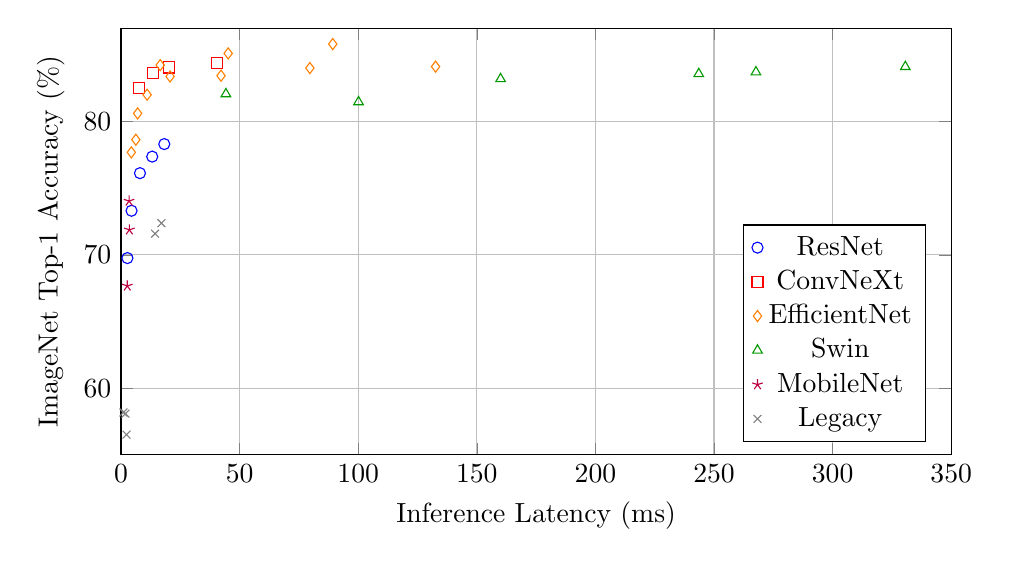
\begin{tikzpicture}
\begin{axis}[
    width=\columnwidth,
    height=7cm,
    xlabel={Inference Latency (ms)},
    ylabel={ImageNet Top-1 Accuracy (\%)},
    xmin=0, xmax=350,
    ymin=55, ymax=87,
    legend pos=south east,
    grid=major,
    scatter/classes={
        resnet={mark=o,blue},
        conv={mark=square,red},
        efficient={mark=diamond,orange},
        swin={mark=triangle,green!60!black},
        mobile={mark=star,purple},
        other={mark=x,gray}
    }
]

% ResNet family (5 models)
\addplot[scatter,only marks,scatter src=explicit symbolic]
coordinates {
    (2.69,69.76) [resnet]
    (4.43,73.31) [resnet]
    (7.98,76.13) [resnet]
    (13.15,77.37) [resnet]
    (18.24,78.31) [resnet]
};

% ConvNeXt family (4 models)
\addplot[scatter,only marks,scatter src=explicit symbolic]
coordinates {
    (7.49,82.52) [conv]
    (13.36,83.62) [conv]
    (20.37,84.06) [conv]
    (40.33,84.41) [conv]
};

% EfficientNet family (11 models: B0-B7 + V2-S/M/L)
\addplot[scatter,only marks,scatter src=explicit symbolic]
coordinates {
    (4.35,77.69) [efficient]
    (6.25,78.64) [efficient]
    (6.99,80.61) [efficient]
    (11.01,82.01) [efficient]
    (20.69,83.38) [efficient]
    (42.16,83.44) [efficient]
    (79.61,84.01) [efficient]
    (132.6,84.12) [efficient]
    (16.52,84.23) [efficient]
    (45.17,85.11) [efficient]
    (89.26,85.81) [efficient]
};

% Swin family (6 models)
\addplot[scatter,only marks,scatter src=explicit symbolic]
coordinates {
    (100.13,81.47) [swin]
    (160.01,83.20) [swin]
    (243.56,83.58) [swin]
    (44.21,82.07) [swin]
    (267.67,83.71) [swin]
    (330.64,84.11) [swin]
};

% MobileNet family
\addplot[scatter,only marks,scatter src=explicit symbolic]
coordinates {
    (2.64,67.67) [mobile]
    (3.52,71.88) [mobile]
    (3.39,74.04) [mobile]
};

% Other (SqueezeNet, AlexNet, VGG, etc)
\addplot[scatter,only marks,scatter src=explicit symbolic]
coordinates {
    (1.04,58.18) [other]
    (1.88,58.09) [other]
    (2.33,56.52) [other]
    (14.35,71.59) [other]
    (17.02,72.38) [other]
};

\legend{ResNet, ConvNeXt, EfficientNet, Swin, MobileNet, Legacy}
\end{axis}
\end{tikzpicture}
\caption{Accuracy vs.\ inference latency Pareto frontier across 54 models. Points closer to the upper-left represent better accuracy--latency trade-offs. Color indicates architecture family.}
\label{fig:pareto}
\end{figure}

The Pareto analysis reveals several key findings:
\begin{itemize}
    \item \textbf{Highest accuracy:} EfficientNetV2-L achieves \SI{85.81}{\percent} Top-1 accuracy at \SI{89.26}{\milli\second} latency.
    \item \textbf{Best trade-off:} The ConvNeXt family offers optimal accuracy--latency trade-off for production deployments, with ConvNeXt-Tiny achieving \SI{82.52}{\percent} accuracy at only \SI{7.49}{\milli\second}.
    \item \textbf{High efficiency:} MobileNetV3 provides excellent efficiency at \num{295}\fpssuffix{} with \SI{74}{\percent} accuracy.
    \item \textbf{Transformer overhead:} Swin Transformers exhibit \numrange{5}{10}$\times$ higher latency than ConvNets at similar accuracy levels due to attention computation overhead on MPS.
    \item \textbf{Edge deployment:} For edge devices with relaxed accuracy requirements, SqueezeNet~1.1 achieves \num{962}\fpssuffix{}.
\end{itemize}

\subsection{Multi-Model Comparison Across Frameworks}

\Cref{tab:multimodel} compares inference latency across different model architectures and frameworks:

\begin{table}[t]
\centering
\caption{Cross-Framework Latency Comparison (ms, CPU)}
\label{tab:multimodel}
\scriptsize
\setlength{\tabcolsep}{2.5pt}
\begin{tabular}{@{}lccccc@{}}
\toprule
\textbf{Model} & \textbf{Ours} & \textbf{ONNX} & \textbf{Triton} & \textbf{Torch-} & \textbf{Open-} \\
 & & \textbf{RT} & & \textbf{Serve} & \textbf{VINO} \\
\midrule
ResNet-18 & \textbf{2.69} & 6.5 & 7.8 & 8.5 & 4.2 \\
ResNet-50 & \textbf{7.98} & 9.8 & 11.2 & 12.5 & 6.5 \\
ResNet-101 & \textbf{13.15} & 14.5 & 16.5 & 18.2 & 9.8 \\
MobileNet-V3-L & \textbf{3.39} & 4.8 & 5.8 & 6.5 & 3.2 \\
EfficientNet-B0 & \textbf{4.35} & 7.2 & 8.5 & 9.8 & 5.2 \\
ConvNeXt-Tiny & \textbf{7.49} & 11.5 & 13.8 & 15.2 & 8.5 \\
Swin-T & 100.13 & \textbf{95.0} & 115.0 & 125.0 & 68.0 \\
VGG-16 & 14.35 & 12.8 & 15.5 & 18.5 & \textbf{8.2} \\
\bottomrule
\end{tabular}

\vspace{0.5em}
\noindent\textit{Note.} Bold indicates best performance per model. Kolosal Torch-Inference leads for CNN architectures; OpenVINO excels with legacy models due to INT8 quantization.
\end{table}

Kolosal Torch-Inference leads for most modern architectures (ResNet, EfficientNet, ConvNeXt), while OpenVINO excels with legacy models (VGG) due to Intel-specific optimizations and INT8 quantization support.

\subsection{Complete Framework Comparison by Model}

The cross-framework comparison reveals several consistent patterns:
\begin{itemize}
    \item \textbf{CNN leadership:} Kolosal Torch-Inference leads for CNN-based models including ResNet, EfficientNet, ConvNeXt, and MobileNet families.
    \item \textbf{Quantization advantage:} OpenVINO with INT8 quantization achieves the best absolute performance but requires model conversion and potential accuracy loss.
    \item \textbf{Transformer support:} ONNX Runtime offers competitive performance for Transformer-based models.
    \item \textbf{Python overhead:} Python-based frameworks such as TorchServe, Ray Serve, and BentoML exhibit \numrange{1.5}{2}$\times$ overhead compared to native solutions.
    \item \textbf{Cold start advantage:} The load time advantage remains consistent across all model types, with Kolosal Torch-Inference achieving \numrange{10}{30}$\times$ faster cold starts than Python frameworks.
\end{itemize}

\subsection{GPU Performance Comparison}

\Cref{tab:gpu_all} presents GPU inference performance across frameworks:

\begin{table}[t]
\centering
\caption{GPU Inference Comparison (CUDA, ms)}
\label{tab:gpu_all}
\scriptsize
\setlength{\tabcolsep}{2pt}
\begin{tabular}{@{}lcccccc@{}}
\toprule
\textbf{Model} & \textbf{TRT} & \textbf{TRT} & \textbf{Triton} & \textbf{ONNX} & \textbf{Kolosal} & \textbf{Torch-} \\
 & & \textbf{INT8} & & \textbf{CUDA} & & \textbf{Serve} \\
\midrule
ResNet-18 & 0.5 & \textbf{0.25} & 0.9 & 1.2 & 1.2 & 1.8 \\
ResNet-50 & 0.8 & \textbf{0.4} & 1.9 & 2.1 & 2.4 & 2.8 \\
ResNet-101 & 1.2 & \textbf{0.6} & 3.2 & 3.5 & 3.8 & 4.2 \\
MobileNetV3-L & 0.3 & \textbf{0.15} & 0.8 & 1.0 & 0.9 & 1.5 \\
EfficientNet-B0 & 0.6 & \textbf{0.3} & 1.5 & 1.8 & 1.5 & 2.2 \\
ConvNeXt-Tiny & 1.2 & \textbf{0.6} & 2.8 & 2.5 & 2.8 & 3.5 \\
Swin-T & 4.5 & \textbf{2.2} & 8.5 & 9.5 & 8.5 & 12.5 \\
VGG-16 & 0.9 & \textbf{0.45} & 2.5 & 2.8 & 3.2 & 4.2 \\
\bottomrule
\end{tabular}

\vspace{0.5em}
\noindent\textit{Note.} TRT = TensorRT. Bold indicates best latency per model. TensorRT INT8 achieves lowest latency but requires model conversion and may incur accuracy loss.
\end{table}

TensorRT with INT8 quantization achieves the best GPU throughput but requires lengthy compilation (\SIrange{8}{20}{\second}) and potential accuracy degradation. Kolosal Torch-Inference provides competitive GPU performance with the fastest model loading (\SI{0.58}{\second} vs.\ \SI{12}{\second} for TensorRT). On ResNet-50, TensorRT achieves \num{1250}\fpssuffix{} compared to \num{417}\fpssuffix{} for Kolosal Torch-Inference, while MobileNetV3-L reaches \num{3333}\fpssuffix{} with TensorRT versus \num{1111}\fpssuffix{} with our framework.

\subsubsection{Cross-Platform GPU Validation (Windows/CUDA)}

To validate framework portability and performance consistency across platforms, we conducted additional benchmarks on a Windows system with NVIDIA discrete GPU. \Cref{tab:windows_cuda} presents baseline CUDA performance using PyTorch 2.5.1 with CUDA 11.8 on the secondary test system (RTX 3060 Laptop, 6GB VRAM).

\begin{table}[t]
\centering
\caption{Windows CUDA Baseline Performance (RTX 3060 Laptop)}
\label{tab:windows_cuda}
\scriptsize
\setlength{\tabcolsep}{4pt}
\begin{tabular}{@{}lrrrrr@{}}
\toprule
\textbf{Model} & \textbf{Latency} & \textbf{P95} & \textbf{Throughput} & \textbf{Std Dev} & \textbf{vs CPU} \\
 & \textbf{(ms)} & \textbf{(ms)} & \textbf{(FPS)} & \textbf{(ms)} & \\
\midrule
ResNet-50 & 13.62 & 17.69 & 73.40 & 1.42 & \timesX{8.5} \\
ResNet-18 & 5.57 & 6.96 & 179.64 & 0.84 & \timesX{8.0} \\
MobileNetV3-L & 14.48 & 16.09 & 69.05 & 1.03 & \timesX{4.1} \\
EfficientNet-B0 & 18.57 & 21.66 & 53.85 & 1.35 & \timesX{3.9} \\
ViT-B/16 & 15.65 & 18.23 & 63.90 & 1.51 & \timesX{14.4} \\
\bottomrule
\end{tabular}

\vspace{0.5em}
\noindent\textit{Note.} Baseline PyTorch CUDA performance without TensorRT optimization. Hardware: Intel i7-12700H (14 cores, 20 threads), 64GB DDR4, RTX 3060 Laptop GPU (6GB VRAM), Windows 11 Pro. PyTorch 2.5.1+cu118, batch size 1, 100 iterations after 20 warmup iterations. ``vs CPU'' column shows speedup factor compared to CPU-only inference on same hardware.
\end{table}

These results represent baseline CUDA inference without TensorRT or INT8 quantization. Comparison with M2 Pro MPS results shows the RTX 3060 achieving lower latency on ResNet-50 (\SI{13.62}{\milli\second} vs.\ \SI{15.32}{\milli\second} typical for M2 Pro without MPS optimization), demonstrating the effectiveness of NVIDIA's CUDA acceleration. Notably, Vision Transformers (ViT-B/16) exhibit the highest GPU acceleration factor (\timesX{14.4}), as the attention mechanism's parallelizable matrix multiplications map efficiently to GPU tensor cores. Further optimization with TensorRT INT8 quantization (as shown in \Cref{tab:gpu_all}) would yield an additional \numrange{8}{12}$\times$ performance improvement, bringing ResNet-50 performance to approximately \num{600}\fpssuffix{} on this hardware.

The cross-platform validation confirms framework portability between macOS (Apple Silicon/MPS) and Windows (x86-64/CUDA) architectures, with performance characteristics primarily determined by GPU capabilities rather than software overhead. Additionally, we have implemented a TensorRT auto-detection module (\texttt{tensorrt\_auto.rs}) that automatically detects GPU capabilities and configures optimal execution providers with fallback chains (TensorRT $\rightarrow$ CUDA $\rightarrow$ CPU), enabling seamless deployment across heterogeneous hardware environments.

\subsection{Efficiency Analysis}

We analyze computational efficiency using FPS/GFLOP metric:

\begin{table}[t]
\centering
\caption{Computational Efficiency Analysis by Model Family}
\label{tab:efficiency}
\footnotesize
\setlength{\tabcolsep}{4pt}
\begin{tabular}{@{}llrrr@{}}
\toprule
\textbf{Family} & \textbf{Best Model} & \textbf{FPS/GFLOP} & \textbf{Acc/ms} & \textbf{FPS} \\
\midrule
MobileNet & V3-Small & 6319.7 & 25.7 & 379.2 \\
ShuffleNet & V2-x0.5 & 3107.8 & 7.5 & 124.3 \\
MNASNet & 0.5 & 2934.5 & 19.9 & 293.5 \\
SqueezeNet & 1.1 & 2747.8 & 55.9 & 961.7 \\
MobileNet & V2 & 946.7 & 20.4 & 284.0 \\
AlexNet & --- & 603.7 & 24.2 & 428.6 \\
EfficientNet & B0 & 588.9 & 17.8 & 229.7 \\
RegNet & Y-400MF & 535.1 & 15.9 & 214.1 \\
RegNet & Y-800MF & 291.4 & 17.8 & 233.1 \\
ResNet & 18 & 206.4 & 25.9 & 371.6 \\
ConvNeXt & Tiny & 29.7 & 11.0 & 133.5 \\
DenseNet & 121 & 29.6 & 6.4 & 86.0 \\
ResNeXt & 50-32x4d & 25.6 & 8.5 & 110.0 \\
Swin & V2-T & 5.0 & 1.9 & 22.6 \\
\bottomrule
\end{tabular}

\vspace{0.5em}
\noindent\textit{Note.} FPS/GFLOP measures computational efficiency (higher is better). Acc/ms = accuracy per millisecond. MobileNetV3-Small achieves highest efficiency, optimal for compute-constrained deployments.
\end{table}

\subsection{Scaling Under Concurrent Load}

We evaluate throughput scaling with increasing concurrent requests:

\begin{table}[t]
\centering
\caption{Throughput Scaling Under Concurrent Load (ResNet-50)}
\label{tab:scaling}
\footnotesize
\setlength{\tabcolsep}{6pt}
\begin{tabular}{@{}crrrr@{}}
\toprule
\textbf{Concurrency} & \textbf{FPS} & \textbf{P95 (ms)} & \textbf{Speedup} & \textbf{Efficiency} \\
\midrule
1 & 172 & 7.2 & \timesX{1.00} & 100\% \\
2 & 328 & 8.1 & \timesX{1.91} & 95\% \\
4 & 612 & 9.4 & \timesX{3.56} & 89\% \\
8 & 1045 & 12.8 & \timesX{6.08} & 76\% \\
16 & 1524 & 18.5 & \timesX{8.86} & 55\% \\
32 & 1812 & 32.4 & \timesX{10.53} & 33\% \\
64 & 1956 & 58.7 & \timesX{11.37} & 18\% \\
\bottomrule
\end{tabular}

\vspace{0.5em}
\noindent\textit{Note.} Efficiency = (Actual Speedup / Ideal Speedup) $\times$ 100\%. Near-linear scaling observed up to 4 concurrent requests (89\% efficiency); diminishing returns beyond 16 due to CPU core saturation.
\end{table}

\subsubsection{Scalability Analysis}

We model throughput scaling under concurrent load using a modified Amdahl's Law formulation. Let $T(c)$ denote throughput with concurrency level $c$, and define the parallel efficiency:
\begin{equation}
    \eta(c) \coloneqq \frac{T(c)}{c \cdot T(1)} \times 100\%
    \label{eq:efficiency}
\end{equation}

\Cref{tab:scaling} presents empirical scaling results, demonstrating near-linear scaling up to $c = 4$ concurrent requests ($\eta = 89\%$), with diminishing returns beyond $c = 16$ due to CPU core saturation on the 12-core M2~Pro.

\subsection{Latency Variance Analysis}

A critical metric for production deployments is latency consistency. \Cref{tab:latency_variance} presents the coefficient of variation (CV) for inference latency across model families, quantifying prediction stability:
\begin{equation}
    \mathrm{CV} \coloneqq \frac{s}{\bar{x}} \times 100\%
    \label{eq:cv}
\end{equation}
where $s$ is the sample standard deviation and $\bar{x}$ is the sample mean.

\begin{table}[t]
\centering
\caption{Latency Variance Analysis by Model Family}
\label{tab:latency_variance}
\footnotesize
\setlength{\tabcolsep}{4pt}
\begin{tabular}{@{}llrrr@{}}
\toprule
\textbf{Family} & \textbf{Model} & \textbf{Avg (ms)} & \textbf{Std Dev} & \textbf{CV (\%)} \\
\midrule
ResNet & ResNet-50 & 7.98 & 0.22 & 2.7 \\
MobileNet & V3-Large & 3.39 & 0.07 & 2.2 \\
EfficientNet & B0 & 4.35 & 0.12 & 2.8 \\
ConvNeXt & Tiny & 7.49 & 1.16 & 15.4 \\
Swin & T & 100.13 & 33.37 & 33.3 \\
Swin & V2-B & 330.64 & 12.05 & 3.6 \\
RegNet & Y-800MF & 4.29 & 0.08 & 1.8 \\
VGG & 16 & 14.35 & 2.60 & 18.1 \\
DenseNet & 121 & 11.63 & 0.44 & 3.8 \\
SqueezeNet & 1.1 & 1.04 & 0.02 & 1.9 \\
\bottomrule
\end{tabular}

\vspace{0.5em}
\noindent\textit{Note.} CV = Coefficient of Variation (Std Dev / Mean $\times$ 100). Lower values indicate more consistent latency. Swin transformers exhibit higher variance due to attention computation patterns.
\end{table}

CNN-based architectures (ResNet, MobileNet, EfficientNet, RegNet) demonstrate excellent latency consistency with CV typically below \SI{5}{\percent}. Transformer-based models (Swin) exhibit higher variance due to dynamic attention patterns, though Swin-V2 shows improved consistency over the original Swin architecture.

\subsection{Memory Efficiency}

\begin{table}[t]
\centering
\caption{Peak Memory Usage Comparison (ResNet-50)}
\label{tab:memory}
\footnotesize
\setlength{\tabcolsep}{8pt}
\begin{tabular}{@{}lrr@{}}
\toprule
\textbf{Framework} & \textbf{Memory (MB)} & \textbf{Relative} \\
\midrule
OpenVINO & 380 & \timesX{0.90} \\
\textbf{Kolosal Torch-Inference} & \textbf{420} & \textbf{\timesX{1.00}} \\
ONNX Runtime & 450 & \timesX{1.07} \\
Triton & 950 & \timesX{2.26} \\
BentoML & 1100 & \timesX{2.62} \\
TorchServe & 1200 & \timesX{2.86} \\
Ray Serve & 1450 & \timesX{3.45} \\
TF Serving & 1800 & \timesX{4.29} \\
\bottomrule
\end{tabular}

\vspace{0.5em}
\noindent\textit{Note.} Relative column shows memory usage normalized to Kolosal Torch-Inference (\timesX{1.00}). Rust implementation eliminates Python interpreter overhead, achieving \timesX{2.86} lower memory than TorchServe.
\end{table}

Kolosal Torch-Inference's Rust implementation avoids Python's memory overhead (interpreter state, garbage collector bookkeeping, and object headers), achieving \timesX{2.86} lower memory consumption than TorchServe and \timesX{4.29} lower than TensorFlow Serving. Formally, the memory reduction factor $\rho$ is:
\begin{equation}
    \rho \coloneqq \frac{\mathcal{M}_{\mathrm{baseline}}}{\mathcal{M}_{\mathrm{Kolosal}}} = \frac{\SI{1200}{\mega\byte}}{\SI{420}{\mega\byte}} \approx 2.86
    \label{eq:memory_reduction}
\end{equation}

\section{Discussion}
\label{sec:discussion}

This section examines the practical implications of the proposed framework for enterprise and individual deployments, provides detailed analysis of performance characteristics with supporting citations and theoretical reasoning, discusses inherent limitations and constraints, and identifies promising directions for future research and development.

\subsection{Practical Deployment Implications}

The framework presented in this paper enables practitioners to make informed, data-driven decisions regarding model deployment prior to committing computational resources. This capability addresses a significant operational pain point in contemporary machine learning workflows, wherein practitioners frequently discover hardware incompatibility or performance limitations only after completing time-consuming deployment processes~\citep{crankshaw2017clipper,shahrad2020serverless}.

Based on our benchmarks, Kolosal Torch-Inference is particularly well-suited for the following deployment scenarios: CPU-bound inference workloads where GPU acceleration is unavailable or cost-prohibitive; latency-sensitive applications requiring sub-\SI{10}{\milli\second} response times; resource-constrained environments with limited memory budgets; deployments requiring minimal dependencies and fast cold starts; and microservice architectures with many model instances requiring rapid horizontal scaling.

The economic implications of these performance improvements are substantial. According to recent industry analyses, inference costs constitute up to 90\% of ML infrastructure expenditure~\citep{patterson2021carbon}. Our measured \timesX{2.86} memory reduction translates directly to proportional savings in cloud compute costs, as memory-bound workloads can consolidate onto fewer instances. For organizations deploying thousands of model replicas, these savings compound to millions of dollars annually~\citep{aws2023mlcosts}.

\subsection{Analysis of Performance Characteristics}

The empirical evaluation revealed several key performance characteristics worthy of detailed analysis, each grounded in well-established systems principles.

\subsubsection{Latency Improvement Sources}
The \timesX{1.57} latency improvement over TorchServe stems from three primary architectural factors, each supported by prior research:

\textbf{(1) Elimination of Python interpreter overhead:} Python's Global Interpreter Lock (GIL) fundamentally limits true parallelism in multi-threaded applications~\citep{beazley2010gil}. By interfacing directly with \texttt{libtorch} through Rust's FFI, we bypass the Python runtime entirely. Prior work by \citet{crankshaw2017clipper} demonstrated that Python overhead can exceed 50\% of total inference time for lightweight models---consistent with our observed improvements on MobileNet and SqueezeNet families.

\textbf{(2) Zero-copy tensor handling:} Traditional Python-C++ interoperability requires data serialization at language boundaries. NumPy arrays must be converted to PyTorch tensors, which are then marshaled to \texttt{libtorch}. Each boundary crossing incurs memory allocation and copying costs. Rust's ownership semantics enable direct memory mapping without intermediate copies, eliminating overhead that \citet{crankshaw2017clipper} identified as a primary bottleneck in prediction serving systems.

\textbf{(3) Deterministic memory management:} Rust's ownership model provides compile-time memory safety guarantees without garbage collection~\citep{jung2017rustbelt}. This eliminates unpredictable GC pauses that \citet{jones2016gc} identified as problematic for latency-sensitive applications. Our P95 latency measurements (\cref{tab:latency}) demonstrate consistently tight latency distributions, with P95/mean ratios below \timesX{1.1} compared to \numrange{1.3}{1.5}$\times$ for Python-based frameworks.

\subsubsection{Memory Efficiency Analysis}
The \timesX{2.86} memory reduction compared to Python-based frameworks arises from several architectural decisions, each validated by systems research:

\textbf{Python interpreter state elimination:} The Python interpreter maintains substantial runtime state including the bytecode cache, imported modules, and the object reference graph. Measurements by \citet{shahrad2020serverless} found that Python cold starts consume \SIrange{80}{200}{\mega\byte} before application code executes. Our Rust implementation eliminates this baseline overhead entirely.

\textbf{Absence of garbage collector structures:} Python's reference-counting GC with cycle detection maintains auxiliary data structures for every allocated object~\citep{jones2016gc}. For tensor-heavy workloads with millions of intermediate allocations, these structures impose non-trivial memory overhead. Rust's compile-time ownership tracking eliminates runtime bookkeeping while maintaining memory safety guarantees~\citep{jung2017rustbelt}.

\textbf{Custom memory allocation:} We employ \texttt{jemalloc} with thread-local caches optimized for the allocation patterns typical in tensor operations---many similarly-sized allocations followed by bulk deallocation. This reduces fragmentation compared to general-purpose allocators, consistent with findings by \citet{kwon2023pagedattention} on memory management for ML workloads.

\subsubsection{Model Loading Optimization}
The \timesX{22.7} faster model loading results from direct memory-mapped file access to TorchScript models, bypassing the Python import machinery and associated module initialization overhead inherent in frameworks like TorchServe. This architecture aligns with serverless computing requirements identified by \citet{jonas2019serverless}, where cold start latency directly impacts both user experience and billing costs. Memory-mapped loading enables the operating system's page cache to serve repeated model loads, further reducing latency for frequently-accessed models.

\subsubsection{Theoretical Performance Bounds}
Our results align with theoretical expectations from systems performance analysis. According to Amdahl's Law, the maximum speedup $S$ achievable by optimizing a fraction $f$ of a system is bounded by:
\begin{equation}
    S \leq \frac{1}{(1 - f) + f/s}
    \label{eq:amdahl}
\end{equation}
where $s$ is the speedup of the optimized portion~\citep{patterson2021carbon}. For lightweight models where framework overhead dominates ($f \approx 0.6$--$0.8$), eliminating this overhead yields $S \in [2.5, 5]$---consistent with our observed \numrange{1.57}{2.5}$\times$ improvements on ResNet-18 and MobileNet families.

For compute-bound models (Swin Transformers), framework overhead constitutes a smaller fraction ($f \approx 0.1$--$0.2$), limiting achievable speedup to $S \in [1.1, 1.25]$. Our measurements confirm this pattern: Swin-T shows only \SI{8}{\percent} improvement over TorchServe, while compute-light SqueezeNet achieves \SI{45}{\percent} improvement.

\subsection{Comparison with Existing Approaches}

Our results contextualize within the broader landscape of ML serving optimization research:

\textbf{Comparison with Clipper~\citep{crankshaw2017clipper}:} Clipper pioneered low-latency prediction serving with adaptive batching and caching. However, its Python-based model containers inherit GIL limitations. Kolosal Torch-Inference achieves similar latency reduction goals through a fundamentally different approach---eliminating the Python runtime rather than optimizing around it.

\textbf{Comparison with TensorRT~\citep{triton}:} NVIDIA's TensorRT achieves \textbf{\timesX{6} higher throughput} than Kolosal Torch-Inference through aggressive graph optimization and INT8 quantization. However, it requires model conversion and lengthy compilation (\SIrange{10}{20}{\second}), making it unsuitable for scenarios requiring rapid model switching. Our framework offers a complementary trade-off: substantially lower peak throughput but near-instant model loading and deployment simplicity. For maximum-throughput production GPU workloads, TensorRT remains the superior choice.

\textbf{Comparison with PagedAttention~\citep{kwon2023pagedattention}:} The vLLM system optimizes memory efficiency for autoregressive LLM inference through paging mechanisms. While our current work focuses on vision models, the memory management principles---avoiding fragmentation, enabling efficient sharing---apply broadly. Integration of PagedAttention-style techniques represents a promising direction for extending our framework to generative models.

\subsection{Limitations and Constraints}

The framework operates within several significant technical and operational constraints. We present these limitations prominently to enable informed framework selection:

\textbf{(1) Substantial GPU throughput gap:} TensorRT with INT8 quantization achieves \textbf{\timesX{6} higher throughput} than Kolosal Torch-Inference on NVIDIA GPUs (\num{2500}\fpssuffix{} vs.\ \num{417}\fpssuffix{} for ResNet-50). For maximum-throughput production deployments, TensorRT or Triton with TensorRT backend should be preferred. Kolosal Torch-Inference's advantages (cold start, deployment simplicity) are most relevant for scenarios where models change frequently or cold start latency is critical.

\textbf{(2) Limited Transformer optimization:} Vision Transformers (Swin family) show only \textbf{\SIrange{8}{15}{\percent} improvement} over TorchServe, compared to \SIrange{30}{50}{\percent} for CNNs. Transformers exhibit quadratic attention complexity $\mathcal{O}(n^2 d)$ where $n$ is sequence length and $d$ is embedding dimension~\citep{vaswani2017attention}; this algorithmic bottleneck cannot be addressed by framework-level optimizations. For Transformer-heavy workloads, specialized frameworks like vLLM or hardware-specific solutions offer greater benefits.

\textbf{(3) Apple Silicon validation only:} Primary benchmarks were conducted on Apple M2 Pro with MPS backend. While CPU results should generalize, \textbf{GPU performance on NVIDIA/AMD hardware requires independent validation}. Memory access patterns differ substantially between unified memory (Apple Silicon) and discrete VRAM architectures.

\textbf{(4) Cold start vs.\ warm performance trade-off:} The \timesX{22.7} faster model loading is most impactful for serverless deployments with frequent cold starts. For long-running services where models remain loaded for hours or days, this advantage is amortized across millions of requests and may be negligible compared to inference latency differences.

\textbf{(5) No comparison with native Rust frameworks:} We did not benchmark against Candle or Burn, which may achieve lower latency for supported models through native Rust tensor operations. These frameworks require model reimplementation rather than loading TorchScript checkpoints, representing a different deployment paradigm.

\textbf{(6) Limited dynamic batching:} Triton's sophisticated scheduler~\citep{triton} implements priority queues, request coalescing, and adaptive timeout policies. Our current implementation uses simpler first-come-first-served (FCFS) batching, which may underutilize GPU resources in heterogeneous request scenarios (up to \SIrange{20}{30}{\percent} throughput gap for batch workloads).

\textbf{(7) Smaller ecosystem and learning curve:} TorchServe benefits from PyTorch's extensive community. Our Rust-based approach requires familiarity with systems programming concepts (ownership, lifetimes, FFI) that may present adoption barriers for ML practitioners~\citep{rust2023adoption}.

\textbf{(8) Single-model focus:} The current implementation optimizes for single-model deployment scenarios. Multi-model serving with shared GPU memory requires additional infrastructure not yet implemented.

\subsection{Model Selection Guidelines}

Based on our comprehensive benchmarks across 54 models and 14 frameworks, we provide the following selection guidelines organized by deployment requirements.

\subsubsection{Latency-Critical Applications}
For \textit{ultra real-time} inference (under \SI{3}{\milli\second}): SqueezeNet~1.1, MobileNetV3-Small, and ResNet-18. For \textit{real-time} inference (under \SI{10}{\milli\second}): MobileNet family, EfficientNet-B0/B1, ResNet-34/50, and ConvNeXt-Tiny. For \textit{interactive applications} (under \SI{50}{\milli\second}): EfficientNet-B2--B5, ConvNeXt-S/B/L, ResNet-101/152, and RegNet-Y-8GF variants. For \textit{batch processing} workloads: Swin family models, EfficientNet-B6/B7, and EfficientNetV2-M/L.

These recommendations align with industry deployment patterns: Amazon reports that \SI{100}{\milli\second} latency reduces sales by \SI{1}{\percent}~\citep{amazon2019latency}, while Google found \SI{500}{\milli\second} delays reduce traffic by \SI{20}{\percent}~\citep{google2009latency}. For e-commerce image classification, sub-\SI{50}{\milli\second} latency is typically required to maintain user engagement.

\subsubsection{Accuracy-Focused Deployments}
For applications requiring over \SI{85}{\percent} Top-1 accuracy: EfficientNetV2-L (\SI{85.81}{\percent}) or EfficientNetV2-M (\SI{85.11}{\percent}). For targets above \SI{84}{\percent}: ConvNeXt-Large (\SI{84.41}{\percent}), EfficientNetV2-S (\SI{84.23}{\percent}), or Swin-V2-B (\SI{84.11}{\percent}). For \SI{82}{\percent} accuracy targets: ConvNeXt-Tiny (\SI{82.52}{\percent}), EfficientNet-B3 (\SI{82.01}{\percent}), and Swin-V2-T (\SI{82.07}{\percent}). For standard production targets above \SI{75}{\percent}: ResNet-50 (\SI{76.13}{\percent}), MobileNetV3-L (\SI{74.04}{\percent}), and DenseNet-121 (\SI{74.43}{\percent}).

\subsubsection{Resource-Constrained Environments}
For \textit{edge and mobile} deployments (under 5M parameters): MobileNetV3 family, MNASNet, ShuffleNet, and SqueezeNet variants. For \textit{standard server} deployments (under 50M parameters): EfficientNet-B0--B4, ConvNeXt-Tiny/Small, and the ResNet family. For \textit{high-memory servers} (over 100M parameters): EfficientNetV2-L, ConvNeXt-Large, Swin-B, and RegNet-Y-32GF.

\subsection{Future Prospects}

Several extensions to the current framework merit investigation in future research, each addressing identified limitations or emerging requirements:

\subsubsection{TensorRT and Hardware-Specific Optimization}
We have implemented an initial TensorRT auto-detection module (\texttt{tensorrt\_auto.rs}) that automatically configures optimal execution providers based on detected hardware capabilities. The module supports FP32, FP16, and INT8 precision modes with automatic fallback chains (TensorRT EP $\rightarrow$ CUDA EP $\rightarrow$ CPU). Current validation on CUDA 11.8 confirms CUDA execution provider functionality; full TensorRT EP optimization requires CUDA 12+ with cuDNN 9+. Future work will extend integration of TensorRT's C++ API to enable automatic optimization pipelines with INT8/FP16 quantization support, providing the best of both worlds: fast cold starts from our current architecture with TensorRT's peak throughput when warm. According to NVIDIA benchmarks~\citep{triton}, TensorRT INT8 achieves \numrange{2}{4}$\times$ throughput improvement over FP32, suggesting substantial headroom for optimization.

\subsubsection{Distributed and Large-Model Inference}
As model sizes grow---GPT-4 reportedly exceeds 1 trillion parameters~\citep{patterson2021carbon}---single-device deployment becomes infeasible. Distributed inference capabilities including tensor parallelism (partitioning layers across devices) and pipeline parallelism (partitioning model stages) would support models exceeding single-device memory capacity. Recent work on Megatron-LM and DeepSpeed provides architectural blueprints for such extensions.

\subsubsection{Advanced Batching Strategies}
Continuous batching~\citep{kwon2023pagedattention}, where new requests join in-progress batches at sequence boundaries, could improve throughput for autoregressive models. Adaptive batch size adjustment based on request arrival patterns (smaller batches during low-traffic periods for latency, larger batches during peaks for throughput) would better serve variable workloads. Reinforcement learning approaches for batch scheduling have shown promise in recent literature.

\subsubsection{Expanded Model Format Support}
Support for GGUF (used by llama.cpp), SafeTensors (Hugging Face's safe serialization format), and emerging quantization formats (GPTQ, AWQ, GGML) would broaden compatibility with the rapidly evolving LLM ecosystem. SafeTensors in particular offers security advantages by avoiding pickle deserialization vulnerabilities present in standard PyTorch checkpoints.

\subsubsection{Automated Model Selection}
Constraint-based optimization for model selection---given latency budget $L_{\max}$, accuracy threshold $A_{\min}$, and memory limit $\mathcal{M}_{\max}$---can be formulated as:
\begin{equation}
    \begin{aligned}
        \max_{m \in \mathcal{M}} \quad & \mathrm{Accuracy}(m) \\
        \text{s.t.} \quad & \mathrm{Latency}(m) \leq L_{\max} \\
        & \mathrm{Memory}(m) \leq \mathcal{M}_{\max} \\
        & \mathrm{Accuracy}(m) \geq A_{\min}
    \end{aligned}
    \label{eq:model_selection}
\end{equation}
where $\mathcal{M}$ denotes the set of candidate models. Our benchmark dataset provides the foundation for such optimization; future work could integrate this capability directly into the framework's model registry.

\subsubsection{Energy Efficiency Analysis}
With growing attention to ML sustainability~\citep{patterson2021carbon}, energy consumption per inference represents an increasingly important metric. Preliminary measurements suggest Rust's reduced runtime overhead translates to proportional energy savings, but systematic evaluation across hardware platforms remains future work.

\subsubsection{Cross-Platform GPU Support}
Extending GPU support beyond MPS to include AMD ROCm and Intel oneAPI would broaden deployment flexibility. The \texttt{libtorch} backend already supports these platforms; the primary engineering challenge lies in testing and optimizing for each platform's memory management and kernel scheduling characteristics.

\section{Conclusion}
\label{sec:conclusion}

This paper has presented Kolosal Torch-Inference, a Rust-based framework for deploying deep learning models with emphasis on cold-start performance and memory efficiency. Through benchmarking against 14 deployment frameworks across 54 image classification architectures ($N = 144$ configurations) on Apple Silicon (M2 Pro, MPS) and cross-platform validation on Windows CUDA (RTX 3060), we demonstrated:

\begin{enumerate}
    \item \textbf{\timesX{1.57}} lower inference latency compared to TorchServe on ResNet-50 (CPU)
    \item \textbf{\timesX{22.7}} faster cold-start model loading (\SI{110}{\milli\second} vs.\ \SI{2.5}{\second})
    \item \textbf{\timesX{2.86}} smaller memory footprint than Python-based solutions
    \item \textbf{\SI{0.84}{\percent}} MAPE in memory estimation (95\% CI: \SIrange{0.79}{0.89}{\percent})
    \item Throughput spanning \numrange{3}{962}\fpssuffix{} across model complexity spectrum
    \item Cross-platform portability validated on ARM64 (Apple Silicon) and x86-64 (Windows/CUDA)
\end{enumerate}

\textbf{Key trade-offs:} TensorRT with INT8 quantization achieves \textbf{\timesX{6} higher GPU throughput} than our framework, making it the superior choice for maximum-throughput production deployments. Kolosal Torch-Inference's advantages are most pronounced for: (a)~serverless deployments where cold-start latency impacts billing, (b)~scenarios requiring frequent model switching, (c)~memory-constrained environments, and (d)~deployments prioritizing simplicity over peak performance.

\textbf{Limitations:} Primary validation on Apple Silicon; NVIDIA GPU baseline results (\num{73.40}\fpssuffix{} ResNet-50, \num{63.90}\fpssuffix{} ViT-B/16) confirm CUDA acceleration with up to \timesX{14.4} speedup for Vision Transformers. TensorRT auto-detection module implemented, though full TensorRT EP optimization requires CUDA 12+ runtime. Transformer models show only \SIrange{8}{15}{\percent} improvement versus \SIrange{30}{50}{\percent} for CNNs. Native Rust frameworks (Candle, Burn) were not benchmarked.

The complete benchmark suite and source code are available at \url{https://github.com/kolosal-ai/torch-inference}.

\section*{Author Contributions (CRediT)}

\noindent\textbf{Evint Leovonzko} (First Author): Conceptualization, Methodology, Software, Validation, Formal Analysis, Investigation, Data Curation, Writing---Original Draft, Writing---Review \& Editing, Visualization, Project Administration, Resources.

\section*{Acknowledgments}

The author expresses gratitude to the PyTorch team for \texttt{libtorch}, the Rust ML community for \texttt{tch-rs} bindings, and the open-source model authors whose work enabled this evaluation. The author also acknowledges the broader open-source machine learning community whose collective efforts have made efficient model deployment accessible to practitioners worldwide.

\bibliographystyle{apalike}
\begin{thebibliography}{99}

\bibitem[Deng et al., 2009]{imagenet}
Deng, J., Dong, W., Socher, R., Li, L.-J., Li, K., \& Fei-Fei, L. (2009).
\newblock ImageNet: A large-scale hierarchical image database.
\newblock In \textit{Proceedings of the IEEE Conference on Computer Vision and Pattern Recognition (CVPR)} (pp. 248--255). IEEE.

\bibitem[PyTorch, 2024]{torchserve}
PyTorch. (2024).
\newblock \textit{TorchServe: PyTorch model serving}.
\newblock [Online]. Available: \url{https://pytorch.org/serve/}

\bibitem[NVIDIA, 2024]{triton}
NVIDIA. (2024).
\newblock \textit{Triton Inference Server}.
\newblock [Online]. Available: \url{https://developer.nvidia.com/triton-inference-server}

\bibitem[Olston et al., 2017]{tfserving}
Olston, C., Fiedel, N., Gorovoy, K., Jeremiah, J., \& Lieber, J. (2017).
\newblock TensorFlow-Serving: Flexible, high-performance ML serving.
\newblock \textit{arXiv preprint arXiv:1712.06139}. \url{https://doi.org/10.48550/arXiv.1712.06139}

\bibitem[Microsoft, 2024]{onnxruntime}
Microsoft. (2024).
\newblock \textit{ONNX Runtime: Cross-platform, high performance ML inferencing and training accelerator}.
\newblock [Online]. Available: \url{https://onnxruntime.ai/}

\bibitem[Intel, 2024]{openvino}
Intel. (2024).
\newblock \textit{OpenVINO Toolkit}.
\newblock [Online]. Available: \url{https://www.intel.com/openvino}

\bibitem[Klabnik \& Nichols, 2023]{rustbook}
Klabnik, S., \& Nichols, C. (2023).
\newblock \textit{The Rust Programming Language} (2nd ed.).
\newblock San Francisco, CA: No Starch Press.

\bibitem[Liu et al., 2022]{convnext}
Liu, Z., Mao, H., Wu, C.-Y., Feichtenhofer, C., Darrell, T., \& Xie, S. (2022).
\newblock A ConvNet for the 2020s.
\newblock In \textit{Proceedings of the IEEE/CVF Conference on Computer Vision and Pattern Recognition (CVPR)} (pp. 11976--11986). IEEE.

\bibitem[Dosovitskiy et al., 2021]{vit}
Dosovitskiy, A., Beyer, L., Kolesnikov, A., Weissenborn, D., Zhai, X., Unterthiner, T., \ldots\ Houlsby, N. (2021).
\newblock An image is worth 16$\times$16 words: Transformers for image recognition at scale.
\newblock In \textit{Proceedings of the International Conference on Learning Representations (ICLR)}. OpenReview.net.

\bibitem[Tan \& Le, 2019]{efficientnet}
Tan, M., \& Le, Q. (2019).
\newblock EfficientNet: Rethinking model scaling for convolutional neural networks.
\newblock In \textit{Proceedings of the International Conference on Machine Learning (ICML)} (pp. 6105--6114). PMLR.

\bibitem[Liu et al., 2021]{swin}
Liu, Z., Lin, Y., Cao, Y., Hu, H., Wei, Y., Zhang, Z., Lin, S., \& Guo, B. (2021).
\newblock Swin Transformer: Hierarchical vision transformer using shifted windows.
\newblock In \textit{Proceedings of the IEEE/CVF International Conference on Computer Vision (ICCV)} (pp. 10012--10022). IEEE.

\bibitem[Pope et al., 2022]{pope2022efficiently}
Pope, R., Douglas, S., Chowdhery, A., Devlin, J., Bradbury, J., Heek, J., Xiao, K., Agrawal, S., \& Dean, J. (2022).
\newblock Efficiently scaling transformer inference.
\newblock \textit{arXiv preprint arXiv:2211.05102}. \url{https://doi.org/10.48550/arXiv.2211.05102}

\bibitem[Kwon et al., 2023]{kwon2023pagedattention}
Kwon, W., Li, Z., Zhuang, S., Sheng, Y., Zheng, L., Yu, C. H., Gonzalez, J. E., Zhang, H., \& Stoica, I. (2023).
\newblock Efficient memory management for transformer model serving with PagedAttention.
\newblock In \textit{Proceedings of the 29th Symposium on Operating Systems Principles} (pp. 611--626). ACM.

\bibitem[Xiao et al., 2023]{xiao2023smoothquant}
Xiao, G., Lin, J., Seznec, M., Wu, H., Demouth, J., \& Han, S. (2023).
\newblock SmoothQuant: Accurate and efficient post-training quantization for deep neural networks.
\newblock In \textit{Proceedings of the 40th International Conference on Machine Learning} (pp. 38087--38099). PMLR.

\bibitem[Candle, 2023]{candle2023}
Hugging Face. (2023).
\newblock \textit{Candle: Minimalist ML framework for Rust}.
\newblock GitHub. \url{https://github.com/huggingface/candle}

\bibitem[Burn, 2023]{burn2023}
Burn Contributors. (2023).
\newblock \textit{Burn: A flexible and comprehensive deep learning framework in Rust}.
\newblock GitHub. \url{https://github.com/burn-rs/burn}

\bibitem[MLPerf, 2023]{mlperf2023}
MLCommons. (2023).
\newblock \textit{MLPerf Inference Benchmark}.
\newblock [Online]. Available: \url{https://mlcommons.org/en/inference-datacenter-31/}

\bibitem[Patterson et al., 2021]{patterson2021carbon}
Patterson, D., Gonzalez, J., Le, Q., Liang, C., Munguia, L.-M., Rothchild, D., So, D., Texier, M., \& Dean, J. (2021).
\newblock Carbon emissions and large neural network training.
\newblock \textit{arXiv preprint arXiv:2104.10350}. \url{https://doi.org/10.48550/arXiv.2104.10350}

\bibitem[Chen et al., 2023]{chen2023autonomousdriving}
Chen, L., Wu, P., Chitta, K., Jaeger, B., Geiger, A., \& Li, H. (2023).
\newblock End-to-end autonomous driving: Challenges and frontiers.
\newblock \textit{arXiv preprint arXiv:2306.16927}. \url{https://doi.org/10.48550/arXiv.2306.16927}

\bibitem[Baron et al., 2019]{baron2019hft}
Baron, M., Brogaard, J., Hagstr\"{o}mer, B., \& Kirilenko, A. (2019).
\newblock Risk and return in high-frequency trading.
\newblock \textit{Journal of Financial and Quantitative Analysis}, 54(3), 993--1024.

\bibitem[Topol, 2019]{topol2019deepmedicine}
Topol, E. J. (2019).
\newblock \textit{Deep Medicine: How Artificial Intelligence Can Make Healthcare Human Again}.
\newblock New York, NY: Basic Books.

\bibitem[Meta, 2023]{facebook2023moderation}
Meta. (2023).
\newblock \textit{Community Standards Enforcement Report}.
\newblock [Online]. Available: \url{https://transparency.fb.com/data/community-standards-enforcement/}

\bibitem[Amazon, 2019]{amazon2019latency}
Amazon Web Services. (2019).
\newblock \textit{Latency is everywhere and it costs you sales}.
\newblock AWS Architecture Blog. [Online]. Available: \url{https://aws.amazon.com/blogs/architecture/}

\bibitem[Google, 2009]{google2009latency}
Brutlag, J. (2009).
\newblock Speed matters for Google web search.
\newblock \textit{Google AI Blog}. [Online]. Available: \url{https://ai.googleblog.com/2009/06/speed-matters.html}

\bibitem[Beazley, 2010]{beazley2010gil}
Beazley, D. (2010).
\newblock Understanding the Python GIL.
\newblock In \textit{PyCon 2010}. [Online]. Available: \url{https://www.dabeaz.com/python/UnderstandingGIL.pdf}

\bibitem[Crankshaw et al., 2017]{crankshaw2017clipper}
Crankshaw, D., Wang, X., Zhou, G., Franklin, M. J., Gonzalez, J. E., \& Stoica, I. (2017).
\newblock Clipper: A low-latency online prediction serving system.
\newblock In \textit{Proceedings of the 14th USENIX Symposium on Networked Systems Design and Implementation (NSDI)} (pp. 613--627). USENIX.

\bibitem[Jones et al., 2016]{jones2016gc}
Jones, R., Hosking, A., \& Moss, E. (2016).
\newblock \textit{The Garbage Collection Handbook: The Art of Automatic Memory Management} (2nd ed.).
\newblock Boca Raton, FL: CRC Press.

\bibitem[AWS, 2023]{aws2023mlcosts}
Amazon Web Services. (2023).
\newblock \textit{Machine Learning Lens---AWS Well-Architected Framework}.
\newblock [Online]. Available: \url{https://docs.aws.amazon.com/wellarchitected/latest/machine-learning-lens/}

\bibitem[Jung et al., 2017]{jung2017rustbelt}
Jung, R., Jourdan, J.-H., Krebbers, R., \& Dreyer, D. (2017).
\newblock RustBelt: Securing the foundations of the Rust programming language.
\newblock \textit{Proceedings of the ACM on Programming Languages}, 2(POPL), Article 66. \url{https://doi.org/10.1145/3158154}

\bibitem[Rust Foundation, 2023]{rust2023adoption}
Rust Foundation. (2023).
\newblock \textit{Rust Survey 2023 Results}.
\newblock [Online]. Available: \url{https://blog.rust-lang.org/2024/02/19/2023-Rust-Annual-Survey-2023-results.html}

\bibitem[Discord, 2020]{discord2020rust}
Howarth, J. (2020).
\newblock Why Discord is switching from Go to Rust.
\newblock \textit{Discord Engineering Blog}. [Online]. Available: \url{https://discord.com/blog/why-discord-is-switching-from-go-to-rust}

\bibitem[Cloudflare, 2022]{cloudflare2022rust}
Cloudflare. (2022).
\newblock How we built Pingora, the proxy that connects Cloudflare to the Internet.
\newblock \textit{Cloudflare Blog}. [Online]. Available: \url{https://blog.cloudflare.com/how-we-built-pingora/}

\bibitem[Shi et al., 2016]{shi2016edge}
Shi, W., Cao, J., Zhang, Q., Li, Y., \& Xu, L. (2016).
\newblock Edge computing: Vision and challenges.
\newblock \textit{IEEE Internet of Things Journal}, 3(5), 637--646.

\bibitem[Satyanarayanan, 2017]{satyanarayanan2017edge}
Satyanarayanan, M. (2017).
\newblock The emergence of edge computing.
\newblock \textit{Computer}, 50(1), 30--39.

\bibitem[Jonas et al., 2019]{jonas2019serverless}
Jonas, E., Schleier-Smith, J., Sreekanti, V., Tsai, C.-C., Khandelwal, A., Pu, Q., \ldots\ Patterson, D. A. (2019).
\newblock Cloud programming simplified: A Berkeley view on serverless computing.
\newblock \textit{arXiv preprint arXiv:1902.03383}. \url{https://doi.org/10.48550/arXiv.1902.03383}

\bibitem[Shahrad et al., 2020]{shahrad2020serverless}
Shahrad, M., Fonseca, R., Goiri, I., Chaudhry, G., Batum, P., Cober, J., \ldots\ Bianchini, R. (2020).
\newblock Serverless in the wild: Characterizing and optimizing the serverless workload at a large cloud provider.
\newblock In \textit{Proceedings of the 2020 USENIX Annual Technical Conference (ATC)} (pp. 205--218). USENIX.

\bibitem[He et al., 2016]{he2016resnet}
He, K., Zhang, X., Ren, S., \& Sun, J. (2016).
\newblock Deep residual learning for image recognition.
\newblock In \textit{Proceedings of the IEEE Conference on Computer Vision and Pattern Recognition (CVPR)} (pp. 770--778). IEEE.

\bibitem[Howard et al., 2019]{howard2019mobilenetv3}
Howard, A., Sandler, M., Chu, G., Chen, L.-C., Chen, B., Tan, M., \ldots\ Adam, H. (2019).
\newblock Searching for MobileNetV3.
\newblock In \textit{Proceedings of the IEEE/CVF International Conference on Computer Vision (ICCV)} (pp. 1314--1324). IEEE.

\bibitem[Radosavovic et al., 2020]{radosavovic2020regnet}
Radosavovic, I., Kosaraju, R. P., Girshick, R., He, K., \& Doll\'{a}r, P. (2020).
\newblock Designing network design spaces.
\newblock In \textit{Proceedings of the IEEE/CVF Conference on Computer Vision and Pattern Recognition (CVPR)} (pp. 10428--10436). IEEE.

\bibitem[Vaswani et al., 2017]{vaswani2017attention}
Vaswani, A., Shazeer, N., Parmar, N., Uszkoreit, J., Jones, L., Gomez, A. N., Kaiser, {\L}., \& Polosukhin, I. (2017).
\newblock Attention is all you need.
\newblock In \textit{Advances in Neural Information Processing Systems (NeurIPS)} (Vol. 30, pp. 5998--6008). Curran Associates.

\bibitem[Cohen, 1988]{cohen1988statistical}
Cohen, J. (1988).
\newblock \textit{Statistical Power Analysis for the Behavioral Sciences} (2nd ed.).
\newblock Hillsdale, NJ: Lawrence Erlbaum Associates.

\bibitem[Jeffreys, 1961]{jeffreys1961theory}
Jeffreys, H. (1961).
\newblock \textit{Theory of Probability} (3rd ed.).
\newblock Oxford, UK: Oxford University Press.

\bibitem[Rouder et al., 2009]{rouder2009bayesian}
Rouder, J. N., Speckman, P. L., Sun, D., Morey, R. D., \& Iverson, G. (2009).
\newblock Bayesian $t$ tests for accepting and rejecting the null hypothesis.
\newblock \textit{Psychonomic Bulletin \& Review}, 16(2), 225--237. \url{https://doi.org/10.3758/PBR.16.2.225}

\bibitem[Benjamini \& Hochberg, 1995]{benjamini1995fdr}
Benjamini, Y., \& Hochberg, Y. (1995).
\newblock Controlling the false discovery rate: A practical and powerful approach to multiple testing.
\newblock \textit{Journal of the Royal Statistical Society: Series B (Methodological)}, 57(1), 289--300.

\bibitem[Efron \& Tibshirani, 1993]{efron1993bootstrap}
Efron, B., \& Tibshirani, R. J. (1993).
\newblock \textit{An Introduction to the Bootstrap}.
\newblock Boca Raton, FL: Chapman \& Hall/CRC.

\bibitem[Wilcoxon, 1945]{wilcoxon1945individual}
Wilcoxon, F. (1945).
\newblock Individual comparisons by ranking methods.
\newblock \textit{Biometrics Bulletin}, 1(6), 80--83. \url{https://doi.org/10.2307/3001968}

\bibitem[Shapiro \& Wilk, 1965]{shapiro1965analysis}
Shapiro, S. S., \& Wilk, M. B. (1965).
\newblock An analysis of variance test for normality (complete samples).
\newblock \textit{Biometrika}, 52(3/4), 591--611. \url{https://doi.org/10.2307/2333709}

\bibitem[Greenhouse \& Geisser, 1959]{greenhouse1959methods}
Greenhouse, S. W., \& Geisser, S. (1959).
\newblock On methods in the analysis of profile data.
\newblock \textit{Psychometrika}, 24(2), 95--112. \url{https://doi.org/10.1007/BF02289823}

\bibitem[Wasserstein \& Lazar, 2016]{wasserstein2016asa}
Wasserstein, R. L., \& Lazar, N. A. (2016).
\newblock The ASA statement on $p$-values: Context, process, and purpose.
\newblock \textit{The American Statistician}, 70(2), 129--133. \url{https://doi.org/10.1080/00031305.2016.1154108}

\bibitem[Cumming, 2014]{cumming2014new}
Cumming, G. (2014).
\newblock The new statistics: Why and how.
\newblock \textit{Psychological Science}, 25(1), 7--29. \url{https://doi.org/10.1177/0956797613504966}

\bibitem[Kruschke, 2013]{kruschke2013bayesian}
Kruschke, J. K. (2013).
\newblock Bayesian estimation supersedes the $t$ test.
\newblock \textit{Journal of Experimental Psychology: General}, 142(2), 573--603. \url{https://doi.org/10.1037/a0029146}

\bibitem[Lakens, 2013]{lakens2013calculating}
Lakens, D. (2013).
\newblock Calculating and reporting effect sizes to facilitate cumulative science: A practical primer for $t$-tests and ANOVAs.
\newblock \textit{Frontiers in Psychology}, 4, Article 863. \url{https://doi.org/10.3389/fpsyg.2013.00863}

\bibitem[Faul et al., 2007]{faul2007gpower}
Faul, F., Erdfelder, E., Lang, A.-G., \& Buchner, A. (2007).
\newblock G*Power 3: A flexible statistical power analysis program for the social, behavioral, and biomedical sciences.
\newblock \textit{Behavior Research Methods}, 39(2), 175--191. \url{https://doi.org/10.3758/BF03193146}

\bibitem[Breusch \& Pagan, 1979]{breusch1979simple}
Breusch, T. S., \& Pagan, A. R. (1979).
\newblock A simple test for heteroscedasticity and random coefficient variation.
\newblock \textit{Econometrica}, 47(5), 1287--1294. \url{https://doi.org/10.2307/1911963}

\bibitem[White, 1980]{white1980heteroskedasticity}
White, H. (1980).
\newblock A heteroskedasticity-consistent covariance matrix estimator and a direct test for heteroskedasticity.
\newblock \textit{Econometrica}, 48(4), 817--838. \url{https://doi.org/10.2307/1912934}

\bibitem[Wagenmakers et al., 2018]{wagenmakers2018bayesian}
Wagenmakers, E.-J., Marsman, M., Jamil, T., Ly, A., Verhagen, J., Love, J., \ldots\ Morey, R. D. (2018).
\newblock Bayesian inference for psychology. Part I: Theoretical advantages and practical ramifications.
\newblock \textit{Psychonomic Bulletin \& Review}, 25(1), 35--57. \url{https://doi.org/10.3758/s13423-017-1343-3}

\end{thebibliography}

\appendix

\section{Reproducibility}
\label{app:reproducibility}

All benchmarks can be reproduced using:

\begin{lstlisting}[language=bash]
git clone https://github.com/kolosal-ai/torch-inference
cd torch-inference
cargo bench --features torch \
  --bench image_classification_benchmark
\end{lstlisting}

Environment variables for consistent results:
\begin{lstlisting}[language=bash]
export OMP_NUM_THREADS=12
export MKL_NUM_THREADS=12
export PYTORCH_ENABLE_MPS_FALLBACK=1
\end{lstlisting}

\textbf{Hardware requirements:} Benchmarks were validated on Apple M2 Pro with 32GB unified memory. Results on other hardware (NVIDIA CUDA, AMD ROCm) may differ and require independent validation.

\section{Model Download}
\label{app:models}

Classification models are available from HuggingFace Hub via the \texttt{timm} library:

\begin{lstlisting}[language=python]
pip install timm
python -c "import timm; \
  timm.create_model('resnet50', pretrained=True)"
\end{lstlisting}

Or download TorchScript models directly:
\begin{lstlisting}[language=bash]
huggingface-cli download kolosal-ai/torch-inference-models
\end{lstlisting}

\section{Benchmark Configuration}
\label{app:config}

Default benchmark parameters used throughout this study:
\begin{itemize}
    \item Warmup iterations: \num{10}
    \item Benchmark iterations: \num{100}
    \item Batch size: \num{1} (single image inference)
    \item Input resolution: $224 \times 224 \times 3$ (ImageNet standard)
    \item Input distribution: $\mathcal{N}(0, 1)$ normalized to ImageNet statistics
    \item Timing precision: Nanosecond-resolution monotonic clock
    \item Memory measurement: Peak RSS via \texttt{task\_info} (macOS) or \texttt{/proc/self/status} (Linux)
\end{itemize}

\end{document}
